
\chapter{微分}
\label{ch:differentials}

\trDifferential{}是一个直观的几何观念，而我们将要找出它的正确的代数刻画。其代数化身有点不直观，因此先从几何的角度来理解\trDifferential{}会有帮助。此外，尽管这些代数陈述显得古怪，诸证明却都不难也不长。你会注意到，这个主题本可以早在我们认识态射与拟凝聚层之时就讲授。我们通常经由一批例子来引入新观念，但这一次，我们将先花相当多的笔墨讨论理论，然后才进入例子。


\section{动机与总体规划}

设 $X$ 是一个「\trSmooth」的 $k$-\trVariety。我们想定义\trTangentBundle。我们将会看到，做这件事的正确方式可以轻而易举地适用于广泛得多的情形。

\begin{itemize}[leftmargin=2.6em,itemsep=2pt,topsep=3pt]
\item 我们将会看到，对\trScheme{}而言，\trCotangentSheaf（cotangent sheaf）比\trTangentBundle{}或\trTangentSheaf{}更为「自然」。这类似于「\trZariski{}\trCotangentSpace{}比\trTangentSpace{}更自然」这一事实（也就是说，若 $A$ 是一个\trRing{}而 $\mathfrak{m}$ 是一个\trMaximalIdeal，则 $\mathfrak{m}/\mathfrak{m}^2$ 比 $(\mathfrak{m}/\mathfrak{m}^2)^{\vee}$ 「更自然」），自 \S13.1 以来我们已反复讨论过这一点。在两种情形下，缘由都在于：我们是通过「空间」上的函数（层）来理解「空间」的，而这与你心目中关于空间的几何图像在某种意义上互为对偶。所以我们将先定义\trCotangentSheaf。（余）\trTangentSpace{}的元素将称为\textbf{（余）\trTangentVector}。
\item 我们本科阶段的直觉会继续奏效——我们可以用\trJacobianMatrix{}进行计算，在本科式计算适用的那些情形里答案也相同，而且我们甚至还有避开 $\delta$ 与 $\epsilon$ 的额外优势。
\item 我们的构造会自动适用于一般的 $X$，哪怕 $X$ 不\trSmooth（甚至压根谈不上「好」，比如连\trFiniteType{}都不是）也照样适用。\trCotangentSheaf{}未必\trLocallyFree，但它仍将是一个\trQCSheaf。
\item 更妙的是，这一构造还会自然而然地以「相对」的方式奏效。对任意 $\pi\colon X\to Y$，我们将定义 $\Omega_\pi=\Omega_{X/Y}$，即 $X$ 上的一个\trQCSheaf——相对微分层（sheaf of relative differentials）。这个层在某一点处的\trFiber{}将是映射的纤维的诸\trCotangentVector。取 $Y=\Spec k$，便特化为此前的情形。其想法是：它把这个族的诸纤维的\trCotangentSheaf{}黏合在一起。图~\ref{fig:relative-tangent-space}便是映射 $X\to Y$ 在一点 $\mathrm{p}\in X$ 处的相对\trTangentSpace{}的草图——它就是纤维的切空间。（\trTangentSpace{}总比\trCotangentSpace{}容易画！）相对（余）\trTangentSpace{}的元素则称为\textbf{相对（余）\trTangentVector}。
\end{itemize}

\begin{figure}[htbp]
\centering
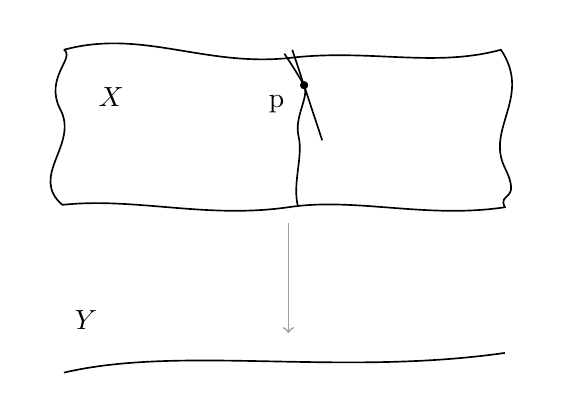
\begin{tikzpicture}[semithick]
  \draw (1.0,5.05)
    .. controls (2.0,5.32) and (2.8,4.82) .. (3.9,4.95)
    .. controls (4.9,5.06) and (5.7,4.82) .. (6.55,5.05)
    .. controls (6.95,4.45) and (6.35,4.05) .. (6.6,3.55)
    .. controls (6.82,3.10) and (6.50,3.25) .. (6.6,3.05)
    .. controls (5.6,2.90) and (4.7,3.18) .. (3.85,3.05)
    .. controls (2.8,2.90) and (1.9,3.18) .. (0.98,3.08)
    .. controls (0.55,3.45) and (1.20,3.85) .. (0.95,4.30)
    .. controls (0.75,4.70) and (1.15,4.95) .. (1.0,5.05);
  \draw (3.80,5.00) .. controls (3.90,4.85) and (3.98,4.72) .. (4.05,4.60)
        .. controls (4.12,4.45) and (3.92,4.20) .. (3.98,3.95)
        .. controls (4.04,3.70) and (3.90,3.35) .. (3.97,3.07);
  \draw (3.90,5.05) -- (4.28,3.90);
  \fill (4.05,4.60) circle (1.5pt);
  \draw[gray!75,->] (3.85,2.85) -- (3.85,1.45);
  \draw (1.0,0.95) .. controls (2.5,1.30) and (4.5,0.90) .. (6.6,1.20);
  \node at (1.60,4.45) {$X$};
  \node at (3.70,4.36) {$\mathrm{p}$};
  \node at (1.28,1.62) {$Y$};
\end{tikzpicture}
\caption{态射 $X\to Y$ 在一点 $\mathrm{p}$ 处的相对\trTangentSpace。（依原书手绘图重绘。）}
\label{fig:relative-tangent-space}
\end{figure}

于是，本章的中心概念便是：对概形的\trMorphism{} $\pi\colon X\to Y$ 而言的\trCotangentSheaf $\Omega_\pi=\Omega_{X/Y}$。在你心目中值得保有的一幅图景如下。若 $\pi\colon X\to Y$ 是\trManifold{}之间的一个\trSubmersion（一个在诸\trTangentSpace{}上诱导满射的映射），你或许会指望：诸纤维在各点 $\mathrm{p}\in X$ 处的\trTangentSpace{}能拼合起来，构成一个\trVectorBundle。这就是（$\pi$ 的）相对\trTangentBundle，而它的\trDual{}就是 $\Omega_{X/Y}$（见图~\ref{fig:relative-tangent-space}）。即使你并不以几何的方式思考问题，你也会发现这很有用。（算术方面的例子，参看\mbox{练习~21.2.H}。）


\section{定义与基本性质}

\textbf{21.2.1. 仿射情形：三个定义。}\quad 我们首先研究仿射情形。设 $A$ 是一个 $B$-代数，于是我们有\trRing{}的一个\trMorphism{} $\phi\colon B\to A$ 与\trScheme{}的一个\trMorphism{} $\Spec A\to\Spec B$。我将用三种方式定义一个 $A$-模 $\Omega_{A/B}$。它称作\textbf{相对\trDifferential{}模}（module of relative differentials）或\textbf{\trKahlerDifferentials{}模}（module of Kähler differentials）。\trDifferential{}模将定义为这个模，连同一条满足下列三条性质的映射 $\mathrm{d}\colon A\to\Omega_{A/B}$。（当心：尽管 $\mathrm{d}$ 把一个 $A$-模送到一个 $A$-模，它一般却不是 $A$-线性的。先验地我们把它当作\trAbelianGroups{}的一个\trHomomorphism，但稍后马上就会让它成为 $B$-模的\trHomomorphism，见\mbox{练习~21.2.A}。）

（i）\emph{可加性}（additivity）：$\mathrm{d}a+\mathrm{d}a'=\mathrm{d}(a+a')$。

（ii）\emph{\trLeibniz}：$\mathrm{d}(aa')=a\,\mathrm{d}a'+a'\,\mathrm{d}a$。

（iii）\emph{在\trPullback{}上的平凡性}（triviality on pullbacks）：对 $b\in\phi(B)$，$\mathrm{d}b=0$。

若你在任何别的语境里见过\trDifferential，这些性质都不会令人惊讶。

\textbf{21.2.A.（平凡练习）}\quad 证明：$\mathrm{d}$ 是 $B$-线性的。

\textbf{21.2.B.（练习）}\quad 证明商法则（quotient rule）：若 $a'=as$，则 $s^2\,\mathrm{d}a=s\,\mathrm{d}a'-a'\,\mathrm{d}s$。

\textbf{21.2.C.（练习）}\quad 叙述并证明 $\mathrm{d}(f(g))$ 的链式法则（chain rule），其中 $f$ 是带 $B$-系数的一个多项式，而 $g\in A$。（作为动机，想一想 $B=k$ 的情形。于是比如 $\mathrm{d}a^n=na^{n-1}\,\mathrm{d}a$，而更一般地，若 $f$ 是一个变元的多项式，则 $\mathrm{d}f(a)=f'(a)\,\mathrm{d}a$，其中 $f'$ 是形式地定义的：若 $f=\sum c_ix^i$，则 $f'=\sum c_iix^{i-1}$。）

现在我们将看到\trKahlerDifferentials{}模的三个定义，它们不久之后就会「层化」为相对\trDifferential{}的层。第一个定义是具体的、可动手操作的。第二个以\trUniversalProperty{}给出。第三个则整体化良好，将使我们在一般情形下也能方便地定义 $\Omega_{X/Y}$。

\textbf{21.2.2. \trDifferential{}的第一个定义：显式描述。}\quad 我们把 $\Omega_{A/B}$ 定义为符号「$\mathrm{d}a$」（$a\in A$）的有限 $A$-线性组合，但须服从上述三条规则（i）--（iii）。例如取 $A=k[x,y]$、$B=k$，那么一个样品\trDifferential{}是 $3x^2\,\mathrm{d}y+4\,\mathrm{d}x\in\Omega_{A/B}$。我们有诸如下列的恒等式：$\mathrm{d}(3xy^2)=3y^2\,\mathrm{d}x+6xy\,\mathrm{d}y$。

\textbf{21.2.3. 关键事实。}\quad 注意，若 $A$ 在 $B$ 上（作为代数）由一些 $x_i\in A$ 生成（其中 $i$ 属于某个指标集，可以无穷），并服从某些关系 $r_j$（其中 $j$ 属于某个指标集，且每条关系都是诸 $x_i$ 的一个多项式），则 $A$-模 $\Omega_{A/B}$ 由诸 $\mathrm{d}x_i$ 生成，且服从关系 $\mathrm{d}r_j=0$。简言之，我们不必取遍 $A$ 的每一个元素，而可以取一个生成集；我们也不必取这些生成元之间的每一条关系，而可以取诸关系的一些生成元。

\textbf{21.2.D.（练习）}\quad 验证\mbox{关键事实~21.2.3}。（如果你愿意，可以用仿射\trConormal{}正合列，即\mbox{定理~21.2.12}，来验证它；不同的人喜欢以不同的顺序梳理这套理论。只须当心不要陷入循环论证。）

特别地：

\textbf{21.2.4.\ \trhProposition。}\ ——\ \emph{若 $A$ 是\trFinitelyGenerated{} $B$-代数，则 $\Omega_{A/B}$ 是一个有限型（即\trFinitelyGenerated{}）的 $A$-模。若 $A$ 是\trFinitelyPresented{} $B$-代数，则 $\Omega_{A/B}$ 是一个\trFinitelyPresented{} $A$-模。}

回忆（\S8.3.13）：称一个环 $A$ 在另一个环 $B$ 上是\emph{\trFinitelyPresented}的，若它能以有限多个生成元与有限多条关系表出：
\[
A=B[x_1,\dots,x_n]/(r_1(x_1,\dots,x_n),\dots,r_j(x_1,\dots,x_n)).
\]
若 $A$ 是\trNoetherian{}的，则「\trFinitelyPresented」与「有限型」是一回事，因为「有限多条关系」是白送的，所以你们大多数人不必在意。

现在我们来看几个例子。这些例子中有三个是环映射特别重要的构件：添加自由变元、取\trLocalization、取商。如果我们知道如何处理这三件事，我们就知道（至少在理论上）如何处理任何环映射。（在 \S10.2 中实际理解\trFiberProduct{}时，它们也曾同样有用。）

\textbf{21.2.5. 例子：取商。}\quad 若 $A=B/I$，则 $\Omega_{A/B}=0$：对一切 $a\in A$，$\mathrm{d}a=0$，因为每个这样的 $a$ 都是 $B$ 中某个元素的像。这应当是可信的；此时不存在「相对\trTangentVector」。

\textbf{21.2.6. 例子：添加变元。}\quad 若 $A=B[x_1,\dots,x_n]$，则 $\Omega_{A/B}=A\,\mathrm{d}x_1\oplus\cdots\oplus A\,\mathrm{d}x_n$。（注意，即使我们添加任意无穷多个未定元，这一论证也适用。）这背后的直观几何使得答案非常合理。仿射 $n$-空间的\trCotangentBundle{}确实应当是秩 $n$ 的自由模。

\textbf{21.2.7. 显式例子：一条仿射平面曲线。}\quad 考虑 $\mathbb{A}^2_k$ 中的平面曲线 $y^2=x^3-x$，其中 $k$ 的\trCharacteristic{}不是 $2$（其图像见图~19.7）。令 $A=k[x,y]/(y^2-x^3+x)$、$B=k$。由\mbox{关键事实~21.2.3}，\trDifferential{}模 $\Omega_{A/B}$ 由 $\mathrm{d}x$ 与 $\mathrm{d}y$ 生成，且服从关系
\[
2y\,\mathrm{d}y=(3x^2-1)\,\mathrm{d}x.
\]
于是在 $y\ne 0$ 的轨迹上，$\mathrm{d}x$ 是一个生成元（因为 $\mathrm{d}y$ 可以用 $\mathrm{d}x$ 表出）。我们得出：在 $y\ne 0$ 的轨迹上，$\widetilde{\Omega}_{A/B}$ 同构于平凡\trLineBundle{}（即\trInvertibleSheaf）。类似地，在 $3x^2-1\ne 0$ 的轨迹上，$\mathrm{d}y$ 是一个生成元。这两块轨迹盖满了整条曲线，因为解 $y=0$ 给出 $x^3-x=0$，即 $x=0$ 或 $\pm 1$，而在这些情形的每一处都有 $3x^2-1\ne 0$。我们已经证明了 $\widetilde{\Omega}_{A/B}$ 是一个\trInvertibleSheaf。

我们可以几何地诠释 $\mathrm{d}x$ 与 $\mathrm{d}y$。\trDifferential{} $\mathrm{d}x$ 在哪里消失？上一段表明它在 $2y\ne 0$ 的块上不消失。在 $3x^2-1\ne 0$ 的块上（$\mathrm{d}y$ 在此是生成元），$\mathrm{d}x=(2y/(3x^2-1))\,\mathrm{d}y$，由此可见 $\mathrm{d}x$ 恰在 $y=0$ 处消失。看着图像，你应当觉得可信。我们已经证明了：$\mathrm{d}x=0$ 恰在这条曲线具有竖直\trTangentVector{}的地方成立。一旦我们能够拉回\trDifferential（\mbox{练习~21.2.K(a)} 或\mbox{定理~21.2.26}），我们就可以把 $\mathrm{d}x$ 诠释为 $x$-轴上一个\trDifferential{}拉回到 $\Spec A$ 的结果（沿向 $x$-轴的\trProjection{}作拉回）。这样做时，利用 $\mathrm{d}x$ 在 $x$-轴上不消失这一事实，我们便可把 $\mathrm{d}x=0$ 的轨迹诠释为\trProjection{}映射发生分支的轨迹。（你能算出 $\mathrm{d}y=0$ 在哪里，并给出几何诠释吗？）

这一讨论适用于更一般的平面曲线。设 $A=k[x,y]/f(x,y)$，为方便起见设 $k=\bar{k}$。那么与上面所给相同的论证表明：$\widetilde{\Omega}_{A/k}$ 在\trOpenSubset{} $\mathrm{D}(\partial f/\partial x)$ 上是秩 $1$ 的自由模，在 $\mathrm{D}(\partial f/\partial y)$ 上亦然。若 $\Spec A$ 是一条正则曲线，则这两个集合盖满整个 $\Spec A$。（反过来，\mbox{练习~13.2.F}——基本上就是正则性的\trJacobianCriterion——给出在诸\trClosedPoint{}处的正则性。进而，这条曲线必定\trReduced，否则由于非既约轨迹是闭的，它将在某个\trClosedPoint{}处非既约，与正则性矛盾。最后，在\trGenericPoint{}处的既约性等价于正则性——底层集合是一个点的概形既约当且仅当它正则。另一种做法是，我们可以援引一个大的结果，即\mbox{事实~13.8.2}，从诸\trClosedPoint{}处的正则性得到\trGenericPoint{}处的正则性。）

另一方面，若这条平面曲线\trSingular，则 $\Omega$ \emph{并非}秩 $1$ 的\trLocallyFreeSheaf。例如，考虑平面曲线 $\Spec A$，其中 $A=\mathbb{C}[x,y]/(y^2-x^3)$，于是
\[
\Omega_{A/\mathbb{C}}=(A\,\mathrm{d}x\oplus A\,\mathrm{d}y)/(2y\,\mathrm{d}y-3x^2\,\mathrm{d}x).
\]
那么 $\Omega_{A/\mathbb{C}}$ 在原点处的\trFiber（由令 $x=y=0$ 算得）秩为 $2$，因为它由 $\mathrm{d}x$ 与 $\mathrm{d}y$ 生成，而不受任何关系约束。

上面的讨论中隐含着下面这道练习，它表明 $\Omega$ 可以用\trJacobianMatrix{}计算。

\textbf{21.2.E.（重要而容易的练习：$\Omega_{A/B}$ 的\trJacobianMatrix{}式描述）}\quad 设
\[
A=B[x_1,\dots,x_n]\big/(f_1,\dots,f_r).
\]
那么
\[
\begin{aligned}
\Omega_{A/B}={}&\biggl(\bigoplus_i A\,\mathrm{d}x_i\biggr)\big/\\
&\bigl(A\,\mathrm{d}f_1+\cdots+A\,\mathrm{d}f_r\bigr)
\end{aligned}
\]
可以诠释为\trJacobianMatrix{} \eqref{eq:jacobian-corank-matrix} 的\trCokernel：
\[
\mathrm{J}\colon A^{\oplus r}\longrightarrow A^{\oplus n}.
\]
（你或许会注意到：若 $\mathrm{J}$ 处处满秩，从而 $A$ 在 $B$ 上\trSmooth，则 $\Omega_{A/B}$ 是\trLocallyFree{}的；详见\mbox{练习~21.2.Q}。）

下一个结果把余切模 $\Omega_{A/B}$ 与在一个（有理）点处的余切空间联系起来。

\textbf{21.2.F.（练习：$\Omega$ 在一个有理点处的\trFiber{}即余切空间）}\quad 设 $B$ 是一个\trFiniteType{} $k$-代数，而 $\mathfrak{m}\subset B$ 是一个剩余域为 $k$ 的\trMaximalIdeal。那么存在 $k$-\trVectorSpace{}的一个同构 $\delta\colon\mathfrak{m}/\mathfrak{m}^2\stackrel{\sim}{\longrightarrow}\Omega_{B/k}\otimes_B k$（其中右边的 $k$ 借同构 $k\stackrel{\sim}{\longleftarrow}B/\mathfrak{m}$成为一个 $B$-模）。提示：二者都是用\trJacobianMatrix{}「算出」的。

（即使没有有限型假设，\mbox{练习~21.2.F} 也成立，尽管此时提示不再适用。欢迎你用 $\Omega_{B/k}$ 的\trUniversalProperty{}证明这个更一般的陈述。但我们用不到它。）

\mbox{推论~21.2.33} 将给出一个颇为不同的证明，并将其推广到 $B/\mathfrak{m}$ 是 $k$ 的\trFiniteFieldExtension{}且可分的情形。它将使我们能够把\trZariski{}余切空间的\trJacobianMatrix{}式描述延拓到剩余域是基域的可分代数扩张（而不仅是基域自身）的\trClosedPoint{}上。

\textbf{21.2.G.（练习）}\quad 设 $X$ 是代数闭域上的一个\trFiniteType{}\trScheme。证明：由 $\mathrm{p}\mapsto\dim\mathrm{T}_{\mathrm{p}}X$ 给出的、从 $X$ 的\trClosedPoint{}到 $\mathbb{Z}^{\ge 0}$ 的函数在\trZariski{}拓扑下\trUpperSemicontinuous{}。（请弄清楚「\trClosedPoint{}集合上的\trZariski{}拓扑」是什么意思；参看 \S8.4.8。）\mbox{推论~21.2.33} 将立即把它推广到一切\trCharacteristic{} $0$ 域与一切有限域。

\textbf{21.2.8. 例子：\trLocalization。}\quad 若 $T$ 是 $B$ 的一个\trMultiplicativeSubset，而 $A=T^{-1}B$，则 $\Omega_{A/B}=0$。理由：由商法则（\mbox{练习~21.2.B}），若 $a=b/t$，则 $\mathrm{d}a=(t\,\mathrm{d}b-b\,\mathrm{d}t)/t^2=0$。若 $A=B_f$，这在直观上是可信的；此时 $\Spec A$ 是 $\Spec B$ 的一个\trOpenSubset，故不应存在相对（余）切向量。

\textbf{21.2.H.（重要练习：域扩张）}\quad 即便对于域的\trFiniteFieldExtension，相对\trDifferential{}这个概念也饶有趣味。换句话说，即便当你把一个既约点映到一个既约点时，\trDifferential{}也可能发生有意思的事情。

（a）设 $K/k$ 是一个可分代数扩张。证明 $\Omega_{K/k}=0$。\emph{切勿}假定 $k$ 是有限扩张！（提示：对任意的 $\alpha\in K$，存在多项式 $f(x)$ 使 $f(\alpha)=0$ 且 $f'(\alpha)\ne 0$。）

（b）设 $k$ 是\trCharacteristic{} $p$ 的域，$K=k(t^p)$、$L=k(t)$。计算 $\Omega_{L/K}$（其中 $K\hookrightarrow L$ 是「显然」的包含映射）。

现在我们稍作深入，讨论两列有用的、由几何激发的正合列。

\textbf{21.2.9.\ \trhTheorem（余切正合列，仿射版本）。}\ ——\ \emph{设 $C\to B\to A$ 是一些环映射。那么存在 $A$-模的一个自然正合列}
\[
A\otimes_B\Omega_{B/C}\xrightarrow{\ a\otimes\mathrm{d}b\mapsto a\,\mathrm{d}b\ }\Omega_{A/C}\xrightarrow{\ \mathrm{d}a\mapsto\mathrm{d}a\ }\Omega_{A/B}\longrightarrow 0.
\]

\begin{figure}[htbp]
\centering
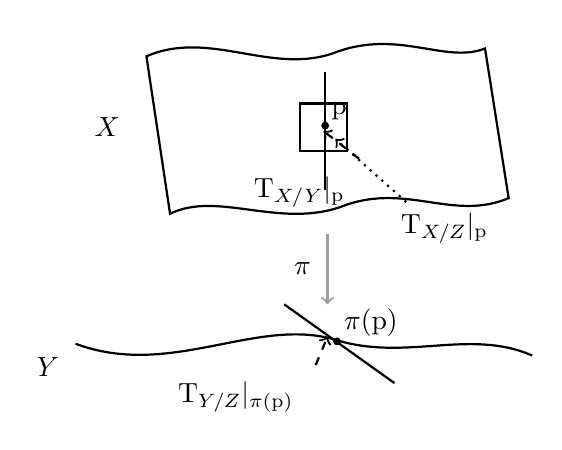
\begin{tikzpicture}[scale=1,line width=0.8pt]
  \draw (0.2,3.2) .. controls (1.0,3.55) and (1.8,2.95) .. (2.6,3.25)
        .. controls (3.4,3.55) and (4.0,3.1) .. (4.5,3.3)
        -- (4.8,1.4)
        .. controls (4.1,1.1) and (3.5,1.6) .. (2.7,1.3)
        .. controls (1.9,1.0) and (1.1,1.5) .. (0.5,1.2)
        -- cycle;
  \node at (-0.3,2.3) {$X$};
  \draw (2.15,2.0) rectangle (2.75,2.6);
  \draw (2.47,1.5) -- (2.47,3.0);
  \fill (2.47,2.32) circle (0.05);
  \node[anchor=south west,inner sep=1pt] at (2.5,2.35) {$\mathrm{p}$};
  \draw[dashed,->] (2.9,1.9) -- (2.45,2.25);
  \node[anchor=north east] at (2.85,1.8) {$\mathrm{T}_{X/Y}|_{\mathrm{p}}$};
  \draw[dotted,->] (3.5,1.35) -- (2.6,2.15);
  \node[anchor=north west] at (3.3,1.35) {$\mathrm{T}_{X/Z}|_{\mathrm{p}}$};
  \draw[->,gray!75] (2.5,0.95) -- (2.5,0.05);
  \node[anchor=east] at (2.42,0.5) {$\pi$};
  \draw (-0.7,-0.45) .. controls (0.5,-0.9) and (1.6,-0.1) .. (2.6,-0.4)
        .. controls (3.5,-0.68) and (4.3,-0.25) .. (5.1,-0.6);
  \draw (1.95,0.05) -- (3.35,-0.95);
  \fill (2.62,-0.42) circle (0.05);
  \node[anchor=south west,inner sep=1pt] at (2.66,-0.4) {$\pi(\mathrm{p})$};
  \node[anchor=north east] at (2.2,-0.8) {$\mathrm{T}_{Y/Z}|_{\pi(\mathrm{p})}$};
  \draw[dashed,->] (2.35,-0.72) -- (2.5,-0.36);
  \node at (-1.05,-0.75) {$Y$};
\end{tikzpicture}
\caption{余切正合列背后的几何。（依原书手绘图重绘。）}\label{fig:cotangent-exact-sequence-geometry}
\end{figure}

这份证明在代数上将相当直接，但这个陈述从根本上来自几何，而记住它的最好方式也正是几何。\cref{fig:cotangent-exact-sequence-geometry} 是一个映射 $\pi\colon X\to Y$ 的草图。这里 $X$ 应当理解为 $\Spec A$，$Y$ 理解为 $\Spec B$，而 $\Spec C$（我们马上会称之为 $Z$）是一个点。（如果你想要一幅 $\Spec C$ 维数更高的图，只须「把\cref{fig:cotangent-exact-sequence-geometry}与一条曲线作积」。）在图中，$Y$ 是「光滑的」，而 $X$ 是「在 $Y$ 上光滑的」——这粗略地说就是所有\trFiber{}都光滑。设 $\mathrm{p}$ 是 $X$ 的一个点。那么 $\pi$ 在 $\mathrm{p}$ 处的\trFiber{}的切空间当然是一个子空间，含于 $X$ 的\trTotalSpace{}在 $\mathrm{p}$ 处的切空间之中。其\trCokernel{}自然就是 $Y$ 在 $\pi(\mathrm{p})$ 处的切空间的拉回。对每个 $\mathrm{p}$ 而言的这个短正合列，应当是 $X$ 上「相对\trTangentSheaf」某个短正合列的一部分：
\[
0\longrightarrow\mathscr{T}_{X/Y}\longrightarrow\mathscr{T}_{X/Z}\longrightarrow\pi^*\mathscr{T}_{Y/Z}\longrightarrow 0
\]
（我们将在 \S21.2.18 中正式定义「相对\trTangentSheaf」。）取对偶便得
\[
0\longrightarrow\pi^*\Omega_{Y/Z}\longrightarrow\Omega_{X/Z}\longrightarrow\Omega_{X/Y}\longrightarrow 0.
\]
这恰好就是\mbox{定理~21.2.9} 的陈述，只不过这里我们还有\trLeftExactness。这一出入是因为定理的陈述更为一般；我们将在\mbox{练习~21.2.S} 中看到，在「光滑」的情形，我们的确有\trLeftExactness。

\textbf{21.2.10.}\ \emph{耐人寻味的注记。}\quad 一如既往，每当你见到某个\trRightExact{}的东西，你就应当怀疑：理应存在某种（上）同调理论，使这个东西是一条\trLongExactSequence{}的末端。事实的确如此，而这条正合列涉及\emph{\trAndre--\trQuillen{}同调}（André--Quillen homology）（详见 [E, p.~386]）。你应当期望左边的下一项是对应于 $A/B$ 的一阶同调，从而特别地不涉及 $C$。于是，如果你已经怀疑在 $A/B$ 与 $B/C$ 都「光滑」（不管这是什么意思）的情形下\trLeftExactness{}成立——此时\cref{fig:cotangent-exact-sequence-geometry} 的直观适用——那么你应当进一步期望：所需的一切只是 $A/B$ 「光滑」，而这将蕴涵第一\trAndre--\trQuillen{}同调应为零。即便你并不确切知道这些词都是什么意思，你也\emph{完全}正确！你还会对\emph{余切复形}（cotangent complex）生出一种隐约的直觉。在「充分光滑」的情形下\trLeftExactness{}成立的例子，见\mbox{命题~21.4.2} 与\mbox{练习~21.2.S}。更一般的陈述见 [Stacks, tag 06B6]。关于此列中接下来两项的清晰讨论，另见 [Liu, Cor.~6.3.22] 与 [Liu, Prop.~6.3.11]：「余切正合列」「\trConormal{}正合列」……

\textbf{21.2.11.}\ \emph{\mbox{定理~21.2.9} 的证明（余切正合列，仿射版本）。}\quad 首先，注意 $\Omega_{A/C}\to\Omega_{A/B}$ 的满性是显然的，因为该映射由 $\mathrm{d}a\mapsto\mathrm{d}a$ 给出（其中 $a\in A$）。

其次，穿过中间项的复合显然是 $0$，因为这个复合由 $a\otimes\mathrm{d}b\mapsto a\mathrm{d}b\mapsto 0$ 给出。

最后，我们希望把 $\Omega_{A/B}$ 识别为 $A\otimes_B\Omega_{B/C}\to\Omega_{A/C}$ 的\trCokernel。$\Omega_{A/B}$ 与 $\Omega_{A/C}$ 恰好相同，只是我们带有额外的关系：对 $b\in B$，$\mathrm{d}b=0$。而这些恰好就是左边 $1\otimes\mathrm{d}b$ 的像。\hfill$\square$

\textbf{21.2.12.\ \trhTheorem（\trConormal{}正合列，仿射版本）。}\ ——\ \emph{设 $B$ 是一个 $C$-代数，$I$ 是 $B$ 的一个\trIdeal，而 $A=B/I$。那么存在 $A$-模的一个自然正合列}
\[
I/I^2\xrightarrow{\ \delta\ }A\otimes_B\Omega_{B/C}\xrightarrow{\ a\otimes\mathrm{d}b\mapsto a\,\mathrm{d}b\ }\Omega_{A/C}\longrightarrow 0.
\]
\emph{映射 $\delta$ 由 $i\mapsto 1\otimes\mathrm{d}i$ 给出，或者更形式化地，$1\otimes\mathrm{d}\colon B/I\otimes_B I\to B/I\otimes_B\Omega_{B/C}$。}

（你会认出映射 $A\otimes_B\Omega_{B/C}\to\Omega_{A/C}$，它来自余切正合列，即\mbox{定理~21.2.9}。映射 $\delta$ 的一个特例曾悄悄出现在\mbox{练习~21.2.F} 中。）这个证明是代数性的，所以其后的几何讨论或有助于澄清你究竟应当如何看待它。

\emph{证明。}\quad 我们将把 $\delta\colon I/I^2\to A\otimes_B\Omega_{B/C}$ 的\trCokernel{}与 $\Omega_{A/C}$ 识别起来。考虑 $A\otimes_B\Omega_{B/C}$。作为 $A$-模，它由 $\mathrm{d}b$（其中 $b\in B$）生成，且服从三种类型的关系：对 $c\in\phi(C)$，$\mathrm{d}c=0$（其中 $\phi\colon C\to B$ 描述了 $B$ 作为 $C$-代数的地位）、可加性，以及\trLeibniz{}法则。给定任何\emph{在 $B$ 中}成立的关系，该关系的 $\mathrm{d}$ 便为 $0$。

现在，$\Omega_{A/C}$ 的定义与之类似，只不过\emph{在 $A$ 中}有更多的关系；而这些恰好就是 $I\subset B$ 的元素。于是我们这样得到 $\Omega_{A/C}$：从 $A\otimes_B\Omega_{B/C}$ 出发，再添加额外的关系 $\mathrm{d}i$（其中 $i\in I$）。但这恰好就是 $\delta$ 的像！（务必看清：$\delta$ 的\trCokernel{}与 $\Omega_{A/C}$ 的这一识别，恰恰正是经由映射 $a\otimes\mathrm{d}b\mapsto a\,\mathrm{d}b$ 实现的。）\hfill$\square$

现在我们来给出\trConormal{}正合列的一个几何诠释，并特别地定义\trConormalSheaf／\trConormal{}层／\trConormal{}丛。

与余切正合列（\mbox{定理~21.2.9}）一样，\trConormal{}正合列从根本上关乎几何。为给出动机，考虑\cref{fig:conormal-exact-sequence-geometry} 的草图。在这幅草图中，一切都是「光滑的」，$X$ 是一维的，$Y$ 是二维的，$j$ 是含入映射 $j\colon X\hookrightarrow Y$\footnote{原书图~21.3 中 $X\to Y$ 的箭头标注作「$\pi$」，而正文明言含入映射为 $j\colon X\hookrightarrow Y$，疑当为「$j$」，兹照录原书。——译者注}，而 $Z$ 是一个点。那么在一点 $\mathrm{p}\in X$ 处，切空间 $\mathscr{T}_X|_{\mathrm{p}}$ 显然单射入 $Y$ 中 $j(\mathrm{p})$ 处的切空间，而其\trCokernel{}便是 $Y$ 中 $X$ 在 $\mathrm{p}$ 处的正规向量空间。这应当给出 $X$ 上诸丛的一个正合列：
\[
0\longrightarrow\mathscr{T}_X\longrightarrow j^*\mathscr{T}_Y\longrightarrow\mathscr{N}_{X/Y}\longrightarrow 0.
\]
取对偶便应当得到
\[
0\longrightarrow\mathscr{N}_{X/Y}^{\vee}\longrightarrow j^*\Omega_{Y/Z}\longrightarrow\Omega_{X/Z}\longrightarrow 0.
\]
这恰好就是定理陈述中出现的内容，只不过：（i）代数几何中的这条正合列不必是\trLeftExact{}的；以及（ii）我们见到的是 $I/I^2$，而非 $\mathscr{N}^{\vee}_{\Spec A/\Spec B}$。

\begin{figure}[htbp]
\centering
\begin{tikzpicture}[scale=1,line width=0.8pt]
  \draw (0.2,1.9) -- (1.0,0.3);
  \node at (-0.25,1.1) {$X$};
  \draw[->,gray] (1.6,1.1) -- (3.0,1.1);
  \node at (2.3,1.45) {$\pi$};
  \draw (3.3,0.1) rectangle (5.7,2.0);
  \draw (3.85,1.85) -- (4.75,0.25);
  \node at (5.35,1.65) {$Y$};
  \draw[->,gray] (4.5,-0.15) -- (4.5,-0.85);
  \fill (4.5,-1.1) circle (0.05);
  \node at (4.85,-1.1) {$Z$};
\end{tikzpicture}
\caption{\trConormal{}正合列背后的几何。（依原书手绘图重绘。）}\label{fig:conormal-exact-sequence-geometry}
\end{figure}

\textbf{21.2.13.}\quad 我们这样解决第一个问题（i）：期望\mbox{定理~21.2.12} 的序列在适当「光滑」的情形下\trLeftExact，而事实的确如此；见\mbox{定理~21.2.31} 与\mbox{注记~21.2.32}。（如果你喜欢\mbox{注记~21.2.10}，你或许能正确猜出好几件事。左边下一项应当是 $A/C$ 的第一\trAndre--\trQuillen{}同调，所以我们应当只需要 $A/C$ 光滑，而 $B$ 应当无关紧要。另外，若 $A=B/I$，那么我们应当期望：$I/I^2$ 就是 $A/B$ 的第一\trAndre--\trQuillen{}同调。）

\textbf{21.2.14.}\ \emph{\trConormalSheaf{}与\trConormal{}层。}\quad 我们这样解决第二个问题（ii）：\emph{宣告} $I/I^2$ 为\textbf{\trConormalSheaf}（conormal module），并将在\mbox{定义~21.2.15} 中把那个显然的类似物定义为\emph{\trConormal{}层}（conormal sheaf）。

这里有一些几何直观，说明我们为何会想把（与 $I/I^2$ 相伴的层）称作\trConormal{}层；它很可能会让你困惑，但也可能带来一点启发。首先，若 $\Spec A$ 是 $\Spec B$ 的一个\trClosedPoint，我们便期望\trConormal{}空间恰为余切空间。而确实，若 $A=B/\mathfrak{m}$，则\trZariski{}余切空间正是 $\mathfrak{m}/\mathfrak{m}^2$。（我们在 \S13.1 中便做过这一微妙的联系。）特别地，早晚会有一天，你会形成一种感觉，明白为何 $\mathbb{A}^2_k=\Spec k[x,y]$ 中原点处的\trConormal（＝余切）空间自然地就是由线性形式 $\alpha x+\beta y$ 构成的空间。但接着考虑 $\Spec k[x,y,z]=\mathbb{A}^3_k$ 中由 $I=(x,y)$ 切出的 $z$-轴。$I/I^2$ 的元素可以写成 $\alpha(z)x+\beta(z)y$，其中 $\alpha(z)$ 与 $\beta(z)$ 是多项式。这就颇有理由应当是 $z$-轴的\trConormal{}空间：当 $z$ 变动时，$x$ 与 $y$ 的系数也随之变动。更一般地，同样的想法提示：$n$-空间内部任何坐标 $k$-平面的\trConormalSheaf／\trConormal{}层都对应于 $I/I^2$。现在考虑 $n$ 维\trManifold{} $Y$ 内部的一个 $k$ 维\trManifold{} $X$，带经典拓扑。我们可以实施同一构造：若 $\mathscr{I}$ 是 $Y$ 中 $X$ 的\trIdealSheaf，则 $\mathscr{I}/\mathscr{I}^2$ 可以与\trConormal{}层（本质上是余正规\trVectorBundle）识别起来，因为解析局部地看，$X\hookrightarrow Y$ 可以与 $\mathbb{R}^k\hookrightarrow\mathbb{R}^n$ 识别。由于这个原因，你或许会希望：在代数几何中，若 $\Spec A\hookrightarrow\Spec B$ 是「光滑」之物含入「光滑」之物的包含映射，则 $I/I^2$ 应当是\trConormalSheaf（或者在应用函子 $\sim$ 之后，\trConormal{}层）。受此启发，我们把余正规定义为\emph{总是} $I/I^2$，然后注意它具有良好的性质（例如\mbox{定理~21.2.12}），但须当心：要动手做出诸如 \S21.2.7 中那样的例子，弄清当我们不处在「光滑」情形时它可能有什么出乎意料的行为。

\textbf{21.2.15.}\ \emph{\trhDefinition{}。}\quad 设 $i\colon X\hookrightarrow Y$ 是概形的一个由\trIdealSheaf{} $\mathscr{I}$ 切出的\trClosedEmbedding。把\textbf{闭嵌入的\trConormal{}层}（conormal sheaf for a closed embedding）定义为 $\mathscr{I}/\mathscr{I}^2$，记作 $\mathscr{N}^{\vee}_{X/Y}$。（拟凝聚理想层的乘积定义于\mbox{练习~15.6.E}。）重要：我们把 $\mathscr{N}^{\vee}_{X/Y}$ 诠释为 $X$ 上的一个拟凝聚层，\textbf{而非}（仅仅是）$Y$ 上的——务必弄明白我们为什么可以这样做。（\mbox{练习~17.1.E} 是一条理由，但它造成的迷惑恐怕比提供的帮助还多。）

把\textbf{正规层}（normal sheaf）定义为其对偶 $\mathscr{N}_{X/Y}:=\mathscr{H}om(\mathscr{N}^{\vee}_{X/Y},\OO_X)$。这个记号并不完美，因为它暗示 $\mathscr{N}$ 的对偶总是 $\mathscr{N}^{\vee}$，而这并不总成立：正如对 $A$-模那样，从模到其双对偶的自然态射并不总是同构。（使此事成立的模称为\textbf{自反的}（reflexive），但我们不会使用这个概念。）

若正规层是有限秩的\trLocallyFreeSheaf，则我们称与之相伴的\trVectorBundle{}为 $Y$ 中 $X$ 的\textbf{正规丛}（normal bundle）。

\textbf{21.2.I.（容易练习）}\quad 对概形的一个\emph{局部闭嵌入} $i\colon X\hookrightarrow Y$，定义\textbf{\trConormal{}层}（conormal sheaf）$\mathscr{N}^{\vee}_{X/Y}$（从而正规层 $\mathscr{N}_{X/Y}$ 也随之而定），它是 $X$ 上的一个拟凝聚层。（务必确认你的定义是良定义的！）

在正则嵌入这个良好的情形中，\trConormal{}层（从而正规层）是有限秩的\trLocallyFreeSheaf（或者更不形式化地说，是一个\trVectorBundle）。特别地，$\mathscr{N}$ 的对偶的确是 $\mathscr{N}^{\vee}$。作为热身，我们先处理重要的余维数 $1$ 情形。

\textbf{21.2.J.（练习：有效\trCartierDivisor{}的正规丛）}\quad 设 $D\subset X$ 是一个有效\trCartierDivisor（\S9.5.1）。证明：\trConormal{}层 $\mathscr{N}^{\vee}_{D/X}$ 是 $\OO(-D)|_D$（从而特别地是一个\trInvertibleSheaf），因而正规层是 $\OO(D)|_D$。这为我们先前在 \S15.6.2 中对有效\trCartierDivisor{}的正规丛所下之定义提供了理据。可能令人惊讶的是：当 $X\cong\mathbb{A}^2$ 而 $D$ 是两条坐标轴之并时（更一般地，当 $X$ 正则而 $D$\trSingular{}时），正规层竟然是局部自由的，因为你也许习惯了「\trTubularNeighborhood」（tubular neighborhood）同构于正规丛的想法。

现在我们来处理一般情形。

\textbf{21.2.16.\ \trhProposition。}\ ——
\emph{（a）若\trIdeal{} $I\subset B$ 由一个\trRegularSequence{} $x_1,\dots,x_r$ 生成，则由
\begin{equation*}\tag{21.2.16.1}\label{eq:regular-sequence-conormal}
(a_1,\dots,a_r)\longmapsto a_1x_1+\cdots+a_rx_r
\end{equation*}
给出的映射 $\gamma\colon(B/I)^{\oplus r}\to I/I^2$ 是一个同构，从而把 $I/I^2$ 描述为 $B/I$ 上秩 $r$ 的自由模、以 $x_1,\dots,x_r$ 为基。
（b）余维数为 $r$ 的正则嵌入的（余）正规层是秩 $r$ 的局部自由层。}

（不需要任何\trNoetherian{}假设。）\mbox{练习~24.6.D} 在「$A$ 包含一个域」这一常用情形中给出了（b）的一个不同的、简短的证明（如果你留心的话，其实（a）也在其内）。

\emph{证明。}\quad（a）显然 \eqref{eq:regular-sequence-conormal} 是满的，所以我们只须证明单性。设 $b_1,\dots,b_r\in B$ 满足 $b_1x_1+\cdots+b_rx_r\in I^2$；我们希望证明 $b_i\in I$ 对一切 $i$ 成立。这是下面两个陈述（$a_k$）与（$b_k$）（二者都取 $1\le k\le r$）的推论。

（$a_k$）：设 $b_1,\dots,b_k\in B$ 满足
\begin{equation*}\tag{21.2.16.2}\label{eq:ak-hypothesis}
b_1x_1+\cdots+b_kx_k\in(x_1,\dots,x_k)^2,
\end{equation*}
则 $b_k\in(x_1,\dots,x_k)$。

（$b_k$）：设 $b_1,\dots,b_{k-1}\in B$ 满足
\begin{equation*}\tag{21.2.16.3}\label{eq:bk-hypothesis}
b_1x_1+\cdots+b_{k-1}x_{k-1}\in(x_1,\dots,x_k)^2,
\end{equation*}
则存在 $d_1,\dots,d_{k-1}\in B$ 使得
\begin{equation*}\tag{21.2.16.4}\label{eq:bk-conclusion}
(b_1-d_1x_k)x_1+\cdots+(b_{k-1}-d_{k-1}x_k)x_{k-1}\in(x_1,\dots,x_{k-1})^2.
\end{equation*}

我们先证（$a_k$）。模去 $(x_1,\dots,x_{k-1})$，\eqref{eq:ak-hypothesis} 就变成 $b_kx_k\in(x_k^2)$。于是（由于依\trRegularSequence{}的定义，$x_k$ 是模 $(x_1,\dots,x_{k-1})$ 意义下的非\trZerodivisor），$b_k$ 在模 $(x_1,\dots,x_{k-1})$ 意义下是 $x_k$ 的倍数，故 $b_k\in(x_1,\dots,x_k)$，正如所愿。

我们接着证（$b_k$）。此时 \eqref{eq:bk-hypothesis} 蕴涵
\[
b_1x_1+\cdots+b_{k-1}x_{k-1}=C+(c_1x_1+\cdots+c_kx_k)x_k
\]
对某些 $c_i\in B$ 与某个 $C\in(x_1,\dots,x_{k-1})^2$ 成立。于是 $0\equiv(c_1x_1+\cdots+c_kx_k)x_k$（模 $(x_1,\dots,x_{k-1})$）。由于 $x_k$ 不是模 $(x_1,\dots,x_{k-1})$ 意义下的\trZerodivisor，我们有
\[
c_1x_1+\cdots+c_kx_k=d_1x_1+\cdots+d_{k-1}x_{k-1}
\]
对某些 $d_1,\dots,d_{k-1}\in B$ 成立。于是
\[
(b_1-d_1x_k)x_1+\cdots+(b_{k-1}-d_{k-1}x_k)x_{k-1}=C\in(x_1,\dots,x_{k-1})^2,
\]
这就给出了 \eqref{eq:bk-conclusion}，正如所愿。

（b）由（a）立得。\hfill$\square$

我们很快会遇到一个相关但更难的事实：若 $\mathscr{I}$ 是一个余维数为 $r$ 的正则嵌入的理想层，则 $\mathscr{I}^n/\mathscr{I}^{n+1}$ 局部自由，因为它就是 $\Sym^n(\mathscr{I}/\mathscr{I}^2)$（\mbox{推论~22.3.9}，或\mbox{练习~24.6.E}）。

\textbf{21.2.17. 第二个定义：\trUniversalProperty。}\quad 这是第二个定义，它在哲理上很重要，以\trUniversalProperty{}给出。当然，这是一个刻画而非定义：凭泛性质式的几句废话，它表明若该模（连同映射 $\mathrm{d}$）存在，则它在相差唯一\trIsomorphism{}的意义下唯一；而此后你仍然需要动手构造它，以确信它存在。

设 $A$ 是一个 $B$-代数，而 $M$ 是一个 $A$-模。\textbf{$A$ 到 $M$ 的 $B$-线性\trDerivation}（$B$-linear derivation of $A$ into $M$）是 $B$-模的一个映射 $\mathrm{d}\colon A\to M$（\emph{不必是} $A$-模的映射），满足\trLeibniz{}法则：$\mathrm{d}(fg)=f\,\mathrm{d}g+g\,\mathrm{d}f$。举一例：设 $B=k$、$A=k[x]$、$M=A$，则 $\mathrm{d}/\mathrm{d}x$ 是一个 $k$-线性\trDerivation。再举一例：若 $B=k$、$A=k[x]$、$M=k$，则 $(\mathrm{d}/\mathrm{d}x)|_0$（「在 $0$ 处取导数值」这一算子）是一个 $k$-线性\trDerivation。

第三个例子是 $\mathrm{d}\colon A\to\Omega_{A/B}$，而且事实上 $\mathrm{d}\colon A\to\Omega_{A/B}$ 就是\emph{$A$ 的泛 $B$-线性\trDerivation}。确切地说，映射 $\mathrm{d}\colon A\to\Omega_{A/B}$ 由下面的\trUniversalProperty{}定义：任何其他 $B$-线性\trDerivation{} $\mathrm{d}'\colon A\to M$ 都唯一地穿过 $\mathrm{d}$：
\begin{tikzcd}
A\ar[rr,"\mathrm{d}'"]\ar[dr,"\mathrm{d}"'] && M\\
& \Omega_{A/B}\ar[ur,"f"']
\end{tikzcd}
其中 $f$ 是 $A$-模的一个映射。（再次注意：$\mathrm{d}$ 与 $\mathrm{d}'$ 未必是 $A$-模的映射——它们只是 $B$-线性的。）凭泛性质式的几句废话，若它存在，便在相差唯一\trIsomorphism{}的意义下唯一。映射 $\mathrm{d}\colon A\to\Omega_{A/B}$ 显然满足这条\trUniversalProperty，基本上就是按定义。

取决于你的大脑如何运转，做接下来两道练习时，你可能更愿意使用第一个（构造性的）定义或第二个（\trUniversalProperty{}式的）定义。

\textbf{21.2.K.（练习）}

（a）\emph{（\trDifferential{}的拉回）}\ 若
\begin{tikzcd}
A' & A\ar[l]\\
B'\ar[u] & B\ar[l]\ar[u]
\end{tikzcd}
是一个交换图表，请描述 $A'$-模的一个自然\trHomomorphism{} $A'\otimes_A\Omega_{A/B}\to\Omega_{A'/B'}$。一个重要的特例是 $B=B'$。

（b）\emph{（\trDifferential{}对基扩张表现良好，仿射情形）}\quad 再若上面的图表是一个「张量图表」（即 $A'\cong B'\otimes_B A$，从而该图表是「余笛卡儿」的（co-Cartesian）），证明 $A'\otimes_A\Omega_{A/B}\to\Omega_{A'/B'}$ 是一个同构。（视你的进路而定，这可能比你预期的更刁钻。）

\textbf{21.2.L.（练习：\trLocalization{}（加强版；较\mbox{例~21.2.8}））}\quad 设 $\phi\colon B\to A$ 是环的一个映射，$S$ 是 $A$ 的一个\trMultiplicativeSubset，$T$ 是 $B$ 的一个\trMultiplicativeSubset{}且 $\phi(T)\subset S$，于是我们有下面的交换图表。
\begin{tikzcd}
S^{-1}A & A\ar[l]\\
T^{-1}B\ar[u] & B\ar[l]\ar[u]
\end{tikzcd}
证明：\mbox{练习~21.2.K(a)} 的\trDifferential{}之拉回 $S^{-1}\Omega_{A/B}\to\Omega_{S^{-1}A/T^{-1}B}$ 是一个同构。（从「相对\trTangentVector」的直观图像看，这应当是可信的。）一个重要情形是 $T=\{1\}$。

\textbf{21.2.M.（练习：域扩张（续）；较\mbox{练习~21.2.H}）}

（a）计算 $\Omega_{K(t)/k}$。（提示：先用 \S21.2.6，接\mbox{练习~21.2.L}。）

（b）若 $K/k$ 由 $t_1,\dots,t_n\in K$ \emph{\trSeparablyGenerated}（也就是说，$t_1,\dots,t_n$ 构成一个\trTranscendenceBase，而 $K/k(t_1,\dots,t_n)$ 是代数且可分的，\S10.5.18），证明：$\Omega_{K/k}$ 是一个自由 $K$-模（即\trVectorSpace），以 $\mathrm{d}t_1,\dots,\mathrm{d}t_n$ 为基。一条可行的进路：对 $k\hookrightarrow k(t_1,\dots,t_n)\hookrightarrow K$ 用余切正合列（\mbox{定理~21.2.9}），证明诸 $\mathrm{d}t_i$ 张成作为 $K$-\trVectorSpace{}的 $\Omega_{K/k}$。棘手之处在于证明诸 $\mathrm{d}t_i$ 线性无关。做法是：证明存在唯一的映射 $\Omega_{K/k}\to K$，把 $\mathrm{d}t_1$ 送到 $1$，而把 $\mathrm{d}t_i$（$i>1$）送到 $0$。先就 $K/k(t_1,\dots,t_n)$ 由单个元素生成的情形做出来；再做有限生成的情形；至于一般情形，则通过在一切有限生成子扩张上定义该映射、并借唯一性证明它们「彼此全相合」来完成。

\textbf{21.2.18. 第三个定义：整体化。}\quad 现在我们想把上述定义对概形的任意态射 $\pi\colon X\to Y$ 整体化。我们可以「逐个仿射地」做这件事；只须确保上面的概念对「仿射集的更换」表现良好。这样，$X$ 上的一支相对\trDifferential{}将是如下数据：对每个仿射 $\mathrm{U}\subset X$，给定一支形如 $\sum a_i\,\mathrm{d}b_i$ 的\trDifferential，而在两个仿射\trOpenSet{}的交 $\mathrm{U}\cap\mathrm{U}'$ 上，给定的两支\trDifferential{}分别以 $\mathrm{U}$ 上的 $\sum a_i\,\mathrm{d}b_i$ 与 $\mathrm{U}'$ 上的 $\sum a'_i\,\mathrm{d}b'_i$ 为代表元，且二者在交叠处相等。不过我们不走这条路，而是换一种做法。我会先给出（看似反直观的）定义，然后告诉你应当如何思考它，最后再回到定义本身。

设 $\pi\colon X\to Y$ 是概形的任意态射。回忆 $\delta\colon X\to X\times_YX$ 是一个局部闭嵌入（\mbox{命题~11.2.1(b)}）。\emph{定义}\textbf{相对\trCotangentSheaf}（relative cotangent sheaf）$\Omega_{X/Y}$（或 $\Omega_\pi$）为对角线的\trConormal{}层 $\mathscr{N}^{\vee}_{X/X\times_YX}$（见 \S21.2.14——而若 $X\to Y$ 是\trSeparated{}的，你甚至无须为\mbox{练习~21.2.I} 担心）。（眼下也是定义\textbf{相对\trTangentSheaf}（relative tangent sheaf）$\mathscr{T}_{X/Y}$ 的好时机：取相对\trCotangentSheaf{}的对偶 $\mathscr{H}om(\Omega_{X/Y},\OO_X)$。若我们在 $k$-概形的范畴中工作，则 $\Omega_{X/k}$ 与 $\mathscr{T}_{X/k}$ 常分别称作 $X$ 的\textbf{\trCotangentSheaf}（cotangent sheaf）与\textbf{\trTangentSheaf}（tangent sheaf）。）

现在我们来定义 $\mathrm{d}\colon\OO_X\to\Omega_{X/Y}$。令 $\mathrm{pr}_1\colon X\times_YX\to X$ 与 $\mathrm{pr}_2\colon X\times_YX\to X$ 为那两个\trProjection。于是在\trOpenSet{} $\mathrm{U}$ 上如下定义 $\mathrm{d}\colon\OO_X\to\Omega_{X/Y}$：
\[
\mathrm{d}f=\mathrm{pr}_2^*f-\mathrm{pr}_1^*f.
\]
（你该如何把 $\mathrm{pr}_2^*f-\mathrm{pr}_1^*f$ 诠释为 $\Omega_{X/Y}$ 的一个\trSection？）

\emph{警告}：$\mathrm{d}$ 不是 $X$ 上诸拟凝聚层之间的态射，尽管按这句话唯一可能有的含义，它\emph{是} $\OO_Y$-线性的。

我们很快会看到：$\mathrm{d}$ 的确是层 $\OO_X$ 的一个\trDerivation（按这句话唯一可能有的含义），同时还会看到，我们的新\trDifferential{}概念在仿射\trOpenSet{}上与旧定义相合，从而把定义整体化了。注意，对任意\trOpenSubset{} $\mathrm{U}\subset X$，$\mathrm{d}$ 诱导出一个映射
\begin{equation*}\tag{21.2.18.1}\label{eq:global-d-sections}
\Gamma(\mathrm{U},\OO_X)\longrightarrow\Gamma(\mathrm{U},\Omega_{X/Y}),
\end{equation*}
我们也称之为 $\mathrm{d}$，并把它诠释为「求导」。

\textbf{21.2.19.}\ \emph{动机。}\quad 在把它与其余几个定义联系起来之前，请先让我试着说服你：这是一个合理的定义。（这段讨论是非形式的、不严格的。）比如说，$Y$ 是一个点，而 $X$ 是一个\trManifold。那么 $X\times X$ 上的\trTangentBundle{} $\mathrm{T}_{X\times X}$ 是 $\mathrm{pr}_1^*\mathrm{T}_X\oplus\mathrm{pr}_2^*\mathrm{T}_X$，其中 $\mathrm{pr}_1$ 与 $\mathrm{pr}_2$ 是从 $X\times X$ 到它的两个因子的\trProjection。把它限制到对角线 $\Delta$ 上，并考察正规丛正合列：
\[
0\longrightarrow\mathrm{T}_\Delta\longrightarrow\mathrm{T}_{X\times X}|_\Delta\longrightarrow\mathscr{N}_{\Delta/X}\longrightarrow 0.
\]
现在，左边的态射把 $v$ 送到 $(v,v)$，于是其\trCokernel{}可以诠释为 $(v,-v)$。这样一来，$\mathscr{N}_{\Delta/X}$ 同构于 $\mathrm{T}_X$。于是我们可以反其道而行：我们知道怎样找出\trNormalBundle{}（或者更精确地说，\trConormal{}层），而我们就可以用它来定义\trTangentBundle{}（或者更精确地说，\trCotangentSheaf）。

\textbf{21.2.20.}\ \emph{再谈动机。}\quad 如果你动手做过\mbox{扩展例题~15.3.4}，你或许会发现这里的许多想法在那里已隐约可见，例如 $\mathrm{pr}_2^*f-\mathrm{pr}_1^*f$，以及在「对角线的理想、模去其平方」之中工作。

\textbf{21.2.21.}\ \emph{在仿射情形中检验。}\quad 现在我们来看看，对于 $\Spec A\to\Spec B$ 这一特殊情形，这一切是如何运作的。此时对角态射 $\delta\colon\Spec A\hookrightarrow\Spec A\otimes_BA$ 对应于 $A\otimes_BA$ 的理想 $I$，它是环映射
\[
\alpha\colon\sum x_i\otimes y_i\longmapsto\sum x_iy_i
\]
的\trKernel。

\textbf{21.2.22.}\quad $A\otimes_BA$ 的理想 $I$ 由形如 $1\otimes a-a\otimes 1$ 的元素生成。理由：若 $\alpha(\sum x_i\otimes y_i)=0$，即 $\sum x_iy_i=0$，则
\[
\sum x_i\otimes y_i=\sum(x_i\otimes y_i-x_iy_i\otimes 1)=\sum(x_i\otimes 1)(1\otimes y_i-y_i\otimes 1).
\]

这个\trDerivation{}是 $\mathrm{d}\colon A\to A\otimes_BA$，$a\mapsto(1\otimes a-a\otimes 1)$（这是 $I$ 的一个元素，取模 $I^2$ 后看待）。（在验证它与我们先前的定义相合之前，我们实在不该把它称作「$\mathrm{d}$」，但我们还是不负责任地就这么叫了。）

我们来检验 $\mathrm{d}$ 的确是一个\trDerivation（\S21.2.17）。显然 $\mathrm{d}$ 是 $B$-线性的，所以我们检验\trLeibniz{}法则：
\begin{align*}
\mathrm{d}(aa')-a\,\mathrm{d}a'-a'\,\mathrm{d}a &= 1\otimes aa'-aa'\otimes 1-a\otimes a'+aa'\otimes 1-a'\otimes a+a'a\otimes 1\\
&= -a\otimes a'-a'\otimes a+a'a\otimes 1+1\otimes aa'\\
&= (1\otimes a-a\otimes 1)(1\otimes a'-a'\otimes 1)\\
&\in I^2.
\end{align*}
于是，由 $\Omega_{A/B}$ 的\trUniversalProperty，我们有 $A$-模的一个自然态射 $\Omega_{A/B}\to I/I^2$。

\textbf{21.2.23.\ \trhTheorem。}\ ——\ \emph{由 $\Omega_{A/B}$ 的\trUniversalProperty{}诱导的自然态射 $f\colon\Omega_{A/B}\to I/I^2$ 是一个同构。}

\emph{证明。}\quad 我们将按如下路线证明。（i）我们将证明 $f$ 是满的，而（ii）我们将描述 $g\colon I/I^2\to\Omega_{A/B}$，使得 $g\circ f\colon\Omega_{A/B}\to\Omega_{A/B}$ 是恒等映射（从而表明 $f$ 是单的）。

（i）映射 $f$ 把 $\mathrm{d}a$ 送到 $1\otimes a-a\otimes 1$，而这类元素生成 $I$（\S21.2.22），故 $f$ 是满的。

（ii）考虑由 $x\otimes y\mapsto x\,\mathrm{d}y$ 定义的映射 $A\otimes_BA\to\Omega_{A/B}$。（由 $\otimes$ 的\trUniversalProperty，这是一个良定义的映射；见 \S1.2.5。）把 $g\colon I/I^2\to\Omega_{A/B}$ 定义为该映射到 $I$ 上的限制。我们须检验这是良定义的，也就是说，$I^2$ 的元素都被送到 $0$，换言之，我们需要：
\[
\Bigl(\sum x_i\otimes y_i\Bigr)\Bigl(\sum x'_j\otimes y'_j\Bigr)=\sum_{i,j}x_ix'_j\otimes y_iy'_j\longmapsto 0
\]
其中 $\sum_i x_iy_i=\sum_j x'_jy'_j=0$。但由\trLeibniz{}法则，
\begin{align*}
\sum_{i,j}x_ix'_j\,\mathrm{d}(y_iy'_j) &= \sum_{i,j}x_ix'_jy_i\,\mathrm{d}y'_j+\sum_{i,j}x_ix'_jy'_j\,\mathrm{d}y_i\\
&= \biggl(\sum_i x_iy_i\biggr)\biggl(\sum_j x'_j\,\mathrm{d}y'_j\biggr)+\biggl(\sum_i x_i\,\mathrm{d}y_i\biggr)\biggl(\sum_j x'_jy'_j\biggr)\\
&= 0.
\end{align*}
于是 $g\circ f$ 的确是恒等映射，因为
\[
\mathrm{d}a\xrightarrow{\ f\ }1\otimes a-a\otimes 1\xrightarrow{\ g\ }1\,\mathrm{d}a-a\,\mathrm{d}1=\mathrm{d}a,
\]
正如所愿。\hfill$\square$

\textbf{21.2.N.（容易练习）}\quad 设 $\pi\colon X\to Y$ 是概形的一个态射，带有开子概形 $\Spec A\subset X$ 与 $\Spec B\subset Y$，且 $\Spec A\subset\pi^{-1}(\Spec B)$。把 $\Omega_{X/Y}|_{\Spec A}$ 与 $\widetilde{\Omega}_{A/B}$ 识别起来，并把 $\mathrm{d}\colon\Gamma(\Spec A,\OO_X)\to\Gamma(\Spec A,\Omega_{X/Y})$ 与 $\mathrm{d}\colon A\to\Omega_{A/B}$ 识别起来。于是，整体构造的确自然地把仿射构造「黏合起来」。

现在我们可以利用「$\Omega$ 在仿射\trOpenSet{}上如何运作」的理解，把先前的诸陈述推广到非仿射的场合。

\textbf{21.2.O.（练习）}\quad 若 $\mathrm{U}\subset X$ 是一个\trOpenSubset，证明：映射 \eqref{eq:global-d-sections} 是一个\trDerivation。

\textbf{21.2.P.（练习）}\quad 设 $\pi\colon X\to Y$ 局部有限型，而 $Y$（从而 $X$）局部\trNoetherian。证明：$\Omega_{X/Y}$ 是 $X$ 上的一个凝聚层。（不妨放松\trNoetherian{}假设以换取较弱的结论。）

\textbf{21.2.Q.（练习）}\quad 设 $\pi\colon X\to Y$ 相对维数 $n$ \trSmooth。证明：$\Omega_{X/Y}$ 是秩 $n$ 的局部自由层。提示：$\Omega$ 的\trJacobianMatrix{}式描述，即\mbox{练习~21.2.E}。

概形的余切正合列与\trConormal{}正合列现在便可直接得出。

\textbf{21.2.24.\ \trhTheorem。}\ ——
\emph{（a）（余切正合列）设}
\begin{tikzcd}
X\ar[r,"\pi"] & Y\ar[r,"\rho"] & Z
\end{tikzcd}
\emph{是概形的态射。那么存在 $X$ 上拟凝聚层的一个正合列}
\[
\pi^*\Omega_{Y/Z}\longrightarrow\Omega_{X/Z}\longrightarrow\Omega_{X/Y}\longrightarrow 0,
\]
\emph{此即\mbox{定理~21.2.9} 的整体化。
（b）（\trConormal{}正合列）设 $\rho\colon Y\to Z$ 是概形的一个态射，而 $\iota\colon X\hookrightarrow Y$ 是一个闭嵌入，带\trConormal{}层 $\mathscr{N}^{\vee}_{X/Y}$。那么存在 $X$ 上拟凝聚层的一个正合列}
\[
\mathscr{N}^{\vee}_{X/Y}\xrightarrow{\ \delta\ }\iota^*\Omega_{Y/Z}\longrightarrow\Omega_{X/Z}\longrightarrow 0,
\]
\emph{此即\mbox{定理~21.2.12} 的整体化。}

\textbf{21.2.R.（练习）}\quad 证明\mbox{定理~21.2.24}。（哪些地方需要检验？）

你应当期望：在适当的光滑性之下，这些正合列也同样左正合（见\mbox{注记~21.2.10} 与 \S21.2.13）。下面的结果是余切正合列的一个重要特例。（\mbox{定理~21.2.31} 将对光滑簇的\trConormal{}正合列给出一个类似的陈述。）

\textbf{21.2.S.（练习：$\pi$ 与 $\rho$ 光滑时余切正合列的左正合性）}\quad 证明：若 $\pi$ 与 $\rho$ 都光滑，则余切正合列左正合。提示：你在\mbox{练习~13.6.D} 中用过的那个 $(m+n)\times(m+n)$ 矩阵是「块上三角」的。

\textbf{21.2.25.}\ \emph{拉回相对微分。}\quad 不出所料，相对微分层可以拉回，并且它在\trBaseChange{}下表现良好。

\textbf{21.2.26.\ \trhTheorem（微分的拉回）。}\ ——
\emph{（a）若}
\begin{tikzcd}
X'\ar[r,"\mu"]\ar[d] & X\ar[d]\\
Y'\ar[r] & Y
\end{tikzcd}
\emph{是概形的一个交换图表，则存在 $X'$ 上拟凝聚层的一个自然\trHomomorphism{} $\mu^*\Omega_{X/Y}\to\Omega_{X'/Y'}$。一个重要的特例是 $Y=Y'$。}
\emph{（b）（$\Omega$ 在\trBaseChange{}下表现良好）再若上面的图表是一个笛卡儿方格（从而 $X'\cong X\times_YY'$），则 $\mu^*\Omega_{X/Y}\to\Omega_{X'/Y'}$ 是一个同构。}

\textbf{21.2.T.（练习）}\quad 由\mbox{练习~21.2.K} 推出\mbox{定理~21.2.26}。（为什么\mbox{练习~21.2.K(a)} 的构造「黏合良好」？）

作为\mbox{定理~21.2.26(b)} 的一个特别情形，相对微分层的\trFiber{}的确就是该\trFiber{}的微分层。这样一来，「微分层」这一概念的确把每支\trFiber{}上的微分「黏合起来」了。

\textbf{21.2.U.（练习）}\quad 设 $\alpha\colon X\to Z$ 与 $\beta\colon Y\to Z$ 是两个态射，而 $\alpha'\colon X\times_ZY\to Y$ 与 $\beta'\colon X\times_ZY\to X$ 是由纤维积诱导的态射。描述一个同构
\[
\Omega_{X\times_ZY/Z}\overset{\sim}{\longleftrightarrow}(\beta')^*\Omega_{X/Z}\oplus(\alpha')^*\Omega_{Y/Z}.
\]
（右边常写作 $\Omega_{X/Z}\boxplus\Omega_{Y/Z}$。）

\textbf{21.2.27. 重要：重访簇的光滑性。}

设 $k$ 是一个域。自 \S13.2.3 以来，我们一直在使用一个颇为别扭的 $k$-光滑性定义，而现在我们要把 $k$-光滑性的定义锻造得更稳健一些。

\textbf{21.2.28.}\ \emph{重新定义。}\quad 若一个 $k$-概形 $X$ 局部有限型、纯维数为 $n$，且 $\Omega_{X/k}$ 是秩 $n$ 的局部自由层，则称它是\textbf{维数 $n$ 的 $k$-光滑}（$k$-smooth of dimension $n$）或\textbf{在 $k$ 上维数 $n$ 光滑}（smooth of dimension $n$ over $k$）的。维数 $n$ 常被省去，而人们可能（也许）会想把某种东西称作光滑的——倘若它是各种维数的光滑之物的（概形论）不交并。

\textbf{21.2.V.（练习）}\quad 证明：\mbox{重新定义~21.2.28} 的 $k$-光滑性与\mbox{定义~13.2.4} 相合。（提示：二者都可以用\trJacobianMatrix{}的\trCokernel{}来描述。）

\textbf{21.2.29.}\ \emph{注记。}\quad 不要多久，我们还将在\mbox{定理~24.8.8} 中重访光滑态射的定义（\mbox{定义~13.6.2}）。

\textbf{21.2.W.}\ \extrahard\ \textbf{（练习：给有复几何背景的读者）}\quad 设 $X$ 是一个复代数\trVariety。证明：$X$ 的解析化 $X^{\mathrm{an}}$（定义于\mbox{练习~7.3.P}）光滑（在微分几何的意义下），当且仅当 $X$ 光滑（在代数几何的意义下，即在 $\mathbb{C}$ 上）。此时，证明复流形 $X^{\mathrm{an}}$ 的复维数（即实维数的一半）是 $\dim X$。提示：\trJacobianCriterion{}在两种场合都适用。

\textbf{21.2.30. 光滑簇之嵌入的\trConormal{}正合列的左正合性。}

正如 \S21.2.13 中所描述的，我们期望\trConormal{}正合列在适当「光滑」的情形下左正合。

\textbf{21.2.31.\ \trhTheorem（光滑簇的\trConormal{}正合列）。}\ ——\ \emph{设 $\iota\colon X\hookrightarrow Y$ 是域 $k$ 上光滑簇的一个闭嵌入，带\trConormal{}层 $\mathscr{N}^{\vee}_{X/Y}$。那么 $\mathscr{N}^{\vee}_{X/Y}$ 局部自由，而\trConormal{}正合列（\mbox{定理~21.2.24(b)}）左正合：}
\begin{equation*}\tag{21.2.31.1}\label{eq:conormal-smooth-left-exact}
0\longrightarrow\mathscr{N}^{\vee}_{X/Y}\xrightarrow{\ \delta\ }\iota^*\Omega_{Y/k}\longrightarrow\Omega_{X/k}\longrightarrow 0
\end{equation*}
\emph{正合。}

取对偶，即应用 $\mathscr{H}om(\cdot,\OO_X)$，我们便得到\textbf{正规正合列}（normal exact sequence）
\[
0\longrightarrow\mathscr{T}_{X/k}\longrightarrow\mathscr{T}_{Y/k}|_X\longrightarrow\mathscr{N}_{X/Y}\longrightarrow 0
\]
（其正合性由\mbox{练习~14.2.I} 保证），而它在几何上更为直观（见\cref{fig:conormal-exact-sequence-geometry} 与\mbox{定理~21.2.12} 证明之后的讨论）。

\textbf{21.2.32.}\ \emph{注记。}\quad 余正规列在更为一般的情形下也左正合。基本上所需要的一切，只是 $\iota\circ g\colon X\to Z$ 的适当光滑性\footnote{原书此处作「$\iota\circ g\colon X\to Z$」，然而按上下文 $g$ 未曾定义，疑当为「$g\circ\iota$」（即 \mbox{定理~21.2.24(b)} 中 $Y\to Z$ 与闭嵌入 $\iota$ 的复合 $X\to Z$）之误，兹照录原书。——译者注}；相关事实见 [Stacks, tag 06B7] 与 [Stacks, tag 06BB]。特别地，$Y$ 的光滑性无关紧要！由此，下面的\mbox{重要推论~21.2.33} 对一般的有限型 $Y$ 也成立。

\emph{证明。}

\textbf{21.2.X.（练习）}\quad 证明：\mbox{定理~21.2.31} 为真，当且仅当它经\trBaseChange{}到 $k$ 的代数闭包 $\bar{k}$ 后为真。提示：证明 \eqref{eq:conormal-smooth-left-exact} 中所有项的构造都与代数域扩张相安无事。\trDifferential{}的情形见\mbox{定理~21.2.26}；\trConormal{}层的情形，则请检验其定义与代数域扩张相安无事。

于是我们可以假定 $k$ 代数闭，从而（由\mbox{练习~13.2.J}）光滑 $k$-概形的\trClosedPoint{}都正则。设 $\mathscr{I}$ 为 $\iota\colon X\hookrightarrow Y$ 的\trIdealSheaf。对任一\trClosedPoint{} $\mathrm{p}\in X$，由\mbox{练习~13.2.M(b)}，$\iota$ 在 $\mathrm{p}$ 的一个开邻域内是正则嵌入。因此 $\iota$ 是正则嵌入。（你明白为什么吗？）于是由\mbox{命题~21.2.16(b)}，$\mathscr{I}/\mathscr{I}^2$ 是秩 $r$ 的局部自由层。由\mbox{练习~6.6.G(a)}，$\ker\delta$ 的诸\trAssociatedPoint{}是 $\mathscr{I}/\mathscr{I}^2$ 的诸\trAssociatedPoint{}的一个子集，所以要证 $\ker\delta=0$，只须在 $\mathscr{I}/\mathscr{I}^2$ 的诸\trAssociatedPoint{}处检验，而这些恰恰就是 $X$ 的诸\trAssociatedPoint（因为 $\mathscr{I}/\mathscr{I}^2$ 局部自由）。

由\mbox{命题~13.2.13}（光滑蕴涵既约），$X$ \trReduced。于是我们只须在 $X$（的诸\trIrreducibleComponent）的诸\trGenericPoint{}处检验（因为 $X$ 没有内嵌点；见 \S6.6.2 或\mbox{练习~6.6.R}）。但这要检验一个右正合的\trVectorSpace{}列的\trLeftExactness（$X$ 既约保证了在\trGenericPoint{}处的茎是\trVectorSpace），而由于左边的维数（即 $X$ 在 $Y$ 中的余维数，由\mbox{命题~21.2.16(b)} 给出）恰是另外两者之差，我们就做完了。\hfill$\square$

\textbf{21.2.33. 重要推论。}\ ——\ \emph{设 $Y$ 是一个光滑 $k$-\trVariety，而 $\mathrm{q}\in Y$ 是一个剩余域 $\kappa(\mathrm{q})$ 在 $k$ 上可分的\trClosedPoint。（若 $\operatorname{char}k=0$ 或 $k$ 是有限域，则自动如此。）那么 $\mathrm{q}\hookrightarrow Y$ 的\trConormal{}正合列给出：$Y$ 在 $\mathrm{q}$ 处的\trZariski{}\trCotangentSpace{}与 $\Omega_{Y/k}$ 在 $\mathrm{q}$ 处的\trFiber{}之间的一个同构。}

\emph{证明。}\quad 对 $X=\mathrm{q}$ 应用\mbox{定理~21.2.31}。注意 $\mathrm{q}$ 的确是一个光滑 $k$-\trVariety（用 $\kappa(\mathrm{q})/k$ 的可分性！），而且 $\Omega_{\mathrm{q}/k}=0$。\hfill$\square$

\textbf{21.2.34.}\ \emph{注记。}\quad 若 $Y$ 光滑，这个结果便把\mbox{练习~21.2.F} 推广到了可分闭点；而且如\mbox{注记~21.2.32} 中所述，就连 $Y$ 的这个光滑性条件也可以去掉。正如\mbox{练习~21.2.F} 的陈述之后所描述的，这有一系列推论。例如，它把\trZariski{}切空间的\trJacobianMatrix{}式描述延拓到了可分闭点。

\textbf{21.2.Y.（练习：较 \S13.2.15）}\quad 设 $\mathrm{p}$ 是 $k$-\trVariety{} $X$ 的一个\trClosedPoint，其剩余域 $\kappa(\mathrm{p})$ 在 $k$ 上可分。由\trBaseChange{} $\Spec\bar{k}\to\Spec k$ 定义 $\pi\colon X_{\bar{k}}:=X\times_k\bar{k}\to X$。设 $\mathrm{q}\in\pi^{-1}(\mathrm{p})$。证明：$X_{\bar{k}}$ 在 $\mathrm{q}$ 处正则，当且仅当 $X$ 在 $\mathrm{p}$ 处正则。


\section{例子}

下面的这些例子按专题组织，而不按难度组织。

\textbf{21.3.1. 曲线的\trGeometricGenus。}\quad 一条（域 $k$ 上的）\trSmooth{}既约射影\trCurve{} $C$ 具有\textbf{\trGeometricGenus}（geometric genus）$\mathrm{h}^0(C,\Omega_{C/k})$。（这将推广到更高的维数，见 \S21.5.3。）它总是有限的，因为 $\Omega_{C/k}$ 是\trCoherentSheaf（\mbox{练习~21.2.P}），而射影 $k$-\trScheme{}上\trCoherentSheaf{}的\trSection{}空间是有限维的（\mbox{定理~18.1.3(i)}）。可叹的是，由下述练习可见，这其实算不上一个新不变量。

\textbf{21.3.A.（容易的练习）}\quad 假设\mbox{奇迹~18.5.2}（即 $\Omega_{C/k}$ 是\trSerre{}对偶化的），证明：对一条\trSmooth{}既约射影\trCurve{} $C$ 而言，\trGeometricGenus{}等于算术亏格，即 $\mathrm{h}^0(C,\Omega_{C/k})=\mathrm{h}^1(C,\OO_C)$。

现在我们来计算一些微分吧！

\textbf{21.3.2. 射影直线。}\quad 作为一个重要的首个例子，考虑 $\mathbb{P}^1_k$，带有通常的射影\trCoordinate{} $x_0$ 与 $x_1$。一如往常，第一张片对应于 $x_0\ne0$，形如 $\Spec k[x_{1/0}]$，其中 $x_{1/0}=x_1/x_0$。第二张片对应于 $x_1\ne0$，形如 $\Spec k[x_{0/1}]$，其中 $x_{0/1}=x_0/x_1$。

两张片都同构于 $\mathbb{A}^1_k$，且 $\Omega_{\mathbb{A}^1_k}\cong\OO_{\mathbb{A}^1_k}$。（更精确地说，$\Omega_{k[x]/k}=k[x]\,\mathrm{d}x$。）于是 $\Omega_{\mathbb{P}^1_k}$ 是一个\trInvertibleSheaf（即\trLineBundle）。$\mathbb{P}^1_k$ 上的诸\trInvertibleSheaf{}皆形如 $\OO(m)$。那么，$\Omega_{\mathbb{P}^1/k}$ 究竟是哪一个\trInvertibleSheaf{}呢？

让我们取第一张片上的一个\trSection，即 $\mathrm{d}x_{1/0}$。它在上面既无\trZeros{}也无\trPole，所以让我们看看它在另一张片上的情形。由于 $x_{1/0}=1/x_{0/1}$，我们有 $\mathrm{d}x_{1/0}=-(1/x_{0/1}^2)\,\mathrm{d}x_{0/1}$。于是这个\trSection{}在 $x_{0/1}=0$ 处有一个二阶极点。故 $\Omega_{\mathbb{P}^1/k}\cong\OO(-2)$。作为推论，我们便证明了 $\mathbb{P}^1_k$ 的\trGeometricGenus{}为 $0$。

注意，若把 $k$ 换成 $\mathbb{Z}$，上面的论证照样奏效：第 15 章的 \trWeilDivisor{}与线丛理论在此适用（$\mathbb{P}^1_\mathbb{Z}$ 是\trFactorial{}的），于是前面的论证几乎不加改动地表明 $\Omega_{\mathbb{P}^1_\mathbb{Z}/\mathbb{Z}}\cong\OO(-2)$。又由于 $\Omega$ 对\trBaseChange{}行为良好（\mbox{定理~21.2.26(b)}），且任何\trScheme{}都映射到 $\Spec\mathbb{Z}$，这便蕴涵：对\emph{任何}基概形 $B$，都有 $\Omega_{\mathbb{P}^1_B/B}\cong\OO_{\mathbb{P}^1_B}(-2)$。

（另外，正如 \S18.5.2 所提示的，这表明 $\Omega_{\mathbb{P}^1/k}$ 是 $\mathbb{P}^1_k$ 的\trCanonical{}层；另见\mbox{例~18.5.4}。不过，鉴于我们尚未证明\trSerreDuality，这一点目前意义不大。）

题外一提：切丛的次数为 $2$ 这一事实，与「毛球定理」（Hairy Ball Theorem）有关（即 [Hat, Thm.~2.28] 的维数 $2$ 情形）。

\textbf{21.3.3. 超椭圆曲线。}\quad 在这一整段关于超椭圆曲线的讨论中，我们假定 $k=\bar{k}$ 且 $\operatorname{char}k\ne2$，从而可以应用 \S19.5 的讨论。考虑由一条正则射影\trCurve{} $C$ 给出的\trDoubleCover{} $\pi\colon C\to\mathbb{P}^1_k$，它在 $2g+2$ 个互不相同的点处\trRamification。我们将使用 \eqref{eq:hyperelliptic-two-affine} 中超椭圆曲线的显式坐标描述。特别地，$\pi$ 在 $0$ 处不\trRamification。由\mbox{定理~19.5.1}，$C$ 的\trGenus{}为 $g$。

\textbf{21.3.B.（练习：超椭圆曲线上的微分）}\quad 可逆层 $\Omega_{C/k}$ 的次数是多少？（提示：取 $x$ 为 $\mathbb{P}^1_k$ 的某张\trCoordinatePatch{}上的一个\trCoordinate。考虑 $C$ 上的 $\pi^*\,\mathrm{d}x$，数一数它的极点与零点。用 \S19.5 的显式坐标。你应当发现：$\pi^*\,\mathrm{d}x$ 有 $2g+2$ 个零点与四个极点，以重数计数，总计为 $2g-2$。）做完这道练习，你就能很好地为 \S21.4 的\trRiemann--\trHurwitz{}公式作好准备。

\textbf{21.3.C.（练习）}\quad 证明 $\mathrm{h}^0(C,\Omega_{C/k})=g$（从而 $C$ 的\trGeometricGenus{}为 $g$），做法如下。

（a）证明：$\Spec k[x,y]/(y^2-f(x))$ 上任一在\trInvolution{} $y\mapsto -y$ 下保持的\trRegular{}\trDifferential{} $\omega$（即 $\Omega_{(k[x,y]/(y^2-f(x)))/k}$ 的一个元素）都是从 $\Spec k[x]$ 上的某个\trDifferential{}拉回的。（提示：为陈述「$\omega/\mathrm{d}x$ 是 $\Spec k[x,y]/(y^2-f(x))$ 上一个在\trInvolution{} $y\mapsto -y$ 下保持的\trRationalFunction」赋予意义，并证明 $\omega/\mathrm{d}x$ 是 $x$ 的\trRationalFunction。）

（b）用（a）证明：任一属于 $\mathrm{H}^0(C,\Omega_{C/k})$ 且在\trInvolution{} $\iota\colon y\mapsto -y$ 下保持的\trDifferential{} $\omega$ 都必是经由 $\pi$ 从 $\mathbb{P}^1$ 拉回的，从而必为零。证明：每个\trDifferential{} $\omega\in\mathrm{H}^0(C,\Omega_{C/k})$ 都满足 $\iota^*\omega=-\omega$。

（c）证明：$\mathrm{d}x/y$ 是 $\Spec k[x,y]/(y^2-f(x))$ 上的一个（\trRegular）\trDifferential。证明：对 $0\le i<g$，$x^i(\mathrm{d}x)/y$ 可延拓为 $C$ 上一个整体\trDifferential{} $\omega_i$（即无极点）。

（d）证明：诸 $\omega_i$（$0\le i<g$）是线性无关的\trDifferential，也就是说，它们在向量空间 $\mathrm{H}^0(C,\Omega_{C/k})$ 中线性无关。（提示：令 $\{p,q\}=\pi^{-1}(0)$。证明 $\omega_i$ 在 $p$ 与 $q$ 两处的\trValuation{}均为 $i$。若 $\omega:=\sum_{j=s}^{g-1}a_j\omega_j$ 是诸 $\omega_i$ 的一个非平凡线性组合，其中 $a_j\in k$ 而 $a_s\ne0$，证明 $\omega$ 在 $p$ 处的\trValuation{}为 $s$，从而 $\omega\ne0$。）

（e）证明：诸 $\omega_i$ 张成诸\trDifferential{}的向量空间 $\mathrm{H}^0(C,\Omega_{C/k})$。（提示：若 $\omega\in\mathrm{H}^0(C,\Omega_{C/k})$，用（d）证明存在唯一的诸 $a_i$，使 $\omega':=\omega-\sum_{i=0}^{g-1}a_i\omega_i$ 在 $p$ 处以阶 $\ge g$ 消失。由（b），$\omega'$ 在 $q$ 处也以同一阶消失。再用\mbox{练习~21.3.B} 证明 $\omega'$ 必为零。）

于是，$\Omega_{C/k}$ 是一个次数为 $2g-2$、带有 $g$ 个\trSection{}的\trInvertibleSheaf。

\textbf{21.3.D.}\ \hard\ \textbf{（练习：通向\trSerre{}对偶）}\quad （日后你或许会把它看作\trSerre{}对偶发挥作用的一个例子。）

（a）证明 $\mathrm{h}^1(C,\Omega_{C/k})=1$。把 $\mathrm{H}^1(C,\Omega_{C/k})$ 的一个生成元诠释为 $x^{-1}\,\mathrm{d}x$。（特别地，拉回映射 $\mathrm{H}^1(\mathbb{P}^1,\Omega_{\mathbb{P}^1/k})\to\mathrm{H}^1(C,\Omega_{C/k})$ 是一个\trIsomorphism。）

（b）描述一个自然的\trPerfectPairing
\[
\mathrm{H}^0(C,\Omega_{C/k})\times\mathrm{H}^1(C,\OO_C)\longrightarrow\mathrm{H}^1(C,\Omega_{C/k}).
\]

在我们显式的坐标下，你可以这样来诠释它。回忆\trHyperelliptic{}\trRiemann--\trHurwitz{}公式（\mbox{定理~19.5.1}）的证明中，$\mathrm{H}^1(C,\OO_C)$ 可被诠释为
\[
\langle y/x,\ y/x^2,\ \dots,\ y/x^g\rangle.
\]
那么，配对
\[
\langle \mathrm{d}x/y,\ x\,\mathrm{d}x/y,\ \dots,\ x^{g-1}\,\mathrm{d}x/y\rangle\times\langle y/x,\ y/x^2,\ \dots,\ y/x^g\rangle\longrightarrow\langle x^{-1}\,\mathrm{d}x\rangle
\]
基本上就是「相乘，然后读出 $x^{-1}\,\mathrm{d}x$ 那一项」。用更高档的话说：「相乘，然后取留数」。（你或许想把它与\mbox{例~18.5.4} 作个比较。）

\textbf{21.3.4. 离散赋值环。}\quad 下面这道练习将用于 \S21.4 中\trRiemann--\trHurwitz{}公式的证明。

\textbf{21.3.E.（练习）}\quad 设\trDVR{} $(A,\mathfrak{m},k)$ 是某个\trFinitelyGenerated{} $k$-代数的\trLocalization。设 $t$ 是 $A$ 的一个\trUniformizer。证明：诸\trDifferential{}是秩 $1$ 的自由模，且由 $\mathrm{d}t$ 生成，即 $\Omega_{A/k}=A\,\mathrm{d}t$，做法如下。（借 \S21.5 中的想法来证明这件事也是可能的。）

（a）证明 $\Omega_{A/k}$ 是一个\trFinitelyGenerated{} $A$-\trModule。

（b）证明 $\langle\mathrm{d}t\rangle=\Omega_{A/k}$，也就是说，$\times\,\mathrm{d}t\colon A\to\Omega_{A/k}$ 是满射，做法如下。设 $\pi$ 是投射 $A\to A/\mathfrak{m}=k$，于是对 $a\in A$，有 $a-\pi(a)\in\mathfrak{m}$。定义 $\sigma(a)=(a-\pi(a))/t$。证明 $\Omega_{A/k}=\langle\mathrm{d}t\rangle+\mathfrak{m}\Omega_{A/k}$，所用的事实是：对每个 $a\in A$，
\[
\mathrm{d}a=\sigma(a)\,\mathrm{d}t+t\,\mathrm{d}\sigma(a).
\]

把\trNakayama{}引理版本~3（\mbox{练习~8.2.G}）应用于 $\langle\mathrm{d}t\rangle\subset\Omega_{A/k}$。（这个论证几乎原封不动地也能用来证明：若 $(A,\mathfrak{m},k)$ 是 $k$ 上某个\trFinitelyGenerated{}代数的\trLocalization，而 $t_1,\dots,t_n$ 生成 $\mathfrak{m}$，则 $\mathrm{d}t_1,\dots,\mathrm{d}t_n$ 生成 $\Omega_{A/k}$。）

（c）由（b），$\Omega_{A/k}$ 是一个\trPrincipal{} $A$-\trModule。证明 $\times\,\mathrm{d}t$ 是单射，做法如下。由离散赋值环上有限生成模的分类（\mbox{注记~6.4.4}），只须证明对一切 $m$ 都有 $t^m\,\mathrm{d}t\ne0$。满射 $A\to A/(t^N)$ 诱导一个映射 $\Omega_{A/k}\to\Omega_{(A/(t^N))/k}$，所以只须证明 $t^m\,\mathrm{d}t$ 在 $\Omega_{(A/(t^N))/k}$ 中非零。证明 $A/(t^N)\cong k[t]/(t^N)$。通常的多项式求导法则给出一个映射 $k[t]/(t^N)\to k[t]/(t^{N-1})$，它是 $k[t]/(t^N)$ 在 $k$ 上的一个\trDerivation，而只要 $N$ 充分大，$t^m\,\mathrm{d}t$ 就不会被映到 $0$。把各块拼在一起，完成证明。（这些想法的延伸可以证明：若 $k$ 上某个\trFinitelyGenerated{}的代数是一个\trRegular\trLocalRing，而 $(A,\mathfrak{m},k)$ 是它的\trLocalization，则 $\Omega_{A/k}$ 是秩 $\dim A$ 的自由模。）

\textbf{21.3.5. 射影空间与欧拉正合列。}\quad 我们接下来考察射影空间 $\mathbb{P}^n_k$ 的诸\trDifferential，或者更一般地，$\mathbb{P}^n_A$ 的诸\trDifferential，其中 $A$ 是任意一个\trRing。由于射影空间由形如 $\mathbb{A}^n_A$ 的\trAffine\trOpenSubset{}所覆盖，而在这些开集上诸\trDifferential{}构成秩 $n$ 的\trLocallyFreeSheaf，所以 $\Omega_{\mathbb{P}^n_A/A}$ 也是一个秩 $n$ 的\trLocallyFreeSheaf。

\textbf{21.3.6.\ \trhTheorem（欧拉正合列）。}\ ——\ \emph{诸\trDifferential{}的层 $\Omega_{\mathbb{P}^n_A/A}$ 满足如下正合列：}
\[
0\longrightarrow\Omega_{\mathbb{P}^n_A/A}\xrightarrow{\ \alpha\ }\OO_{\mathbb{P}^n_A}(-1)^{\oplus(n+1)}\xrightarrow{\ \phi\ }\OO_{\mathbb{P}^n_A}\longrightarrow 0.
\]

这条正合列很称手，因为你可以借它以一种具体的方式把握住 $\Omega_{\mathbb{P}^n_A/A}$。应用见\mbox{练习~21.5.Q}。将这条正合列取对偶，我们便得到正合列
\[
0\longrightarrow\OO_{\mathbb{P}^n_A}\xrightarrow{\ \phi^\vee\ }\OO_{\mathbb{P}^n_A}(1)^{\oplus(n+1)}\longrightarrow\mathscr{T}_{\mathbb{P}^n_A/A}\longrightarrow 0.
\]

\textbf{21.3.7.}\ \hard\ \emph{\mbox{定理~21.3.6} 的证明。}\quad 这个证明的真正要点是：我们考虑 $\mathbb{A}^{n+1}_A\setminus\{0\}$ 上那些作为 $\mathbb{P}^n_A$ 上\trDifferential{}之拉回的\trDifferential。若想从 Koszul 复形（\S24.4.1 将简要提到）的角度另找一个解释，见 [E, \S17.5]。

我们先来描述一个映射 $\phi\colon\OO(-1)^{\oplus(n+1)}\to\OO$，稍后再把它的\trKernel{}与 $\Omega_{\mathbb{P}^n_A/A}$ 识别起来。该映射由
\[
\phi\colon(s_0,s_1,\dots,s_n)\longmapsto x_0s_0+x_1s_1+\cdots+x_ns_n.
\]
给出。（你能看出为什么吗？）你应当把它看作一个「次数 $1$」的映射，因为每个 $x_i$ 的次数都是 $1$。

\textbf{21.3.8.\ \trhRemark。}\quad $\phi$ 的\trDual{} $\phi^\vee\colon\OO\to\OO(1)^{\oplus(n+1)}$ 借\mbox{重要定理~15.2.2}（到射影空间的映射）给出一个映射 $\mathbb{P}^n\to\mathbb{P}^n$。这个映射是恒等映射，而这也是以一种「自然」（无坐标）的方式描述 $\phi$ 的途径之一。

\textbf{21.3.F.（容易的练习）}\quad 证明 $\phi$ 是满射，办法是在诸开集 $\mathrm{D}(x_i)$ 上逐一验证。（存在一行字的解法。）

现在我们必须把 $\phi$ 的\trKernel{}与诸\trDifferential{}识别起来。这件事可以在每一块 $\mathrm{D}(x_i)$ 上完成，只要我们所做的方式能对每个开集同时奏效即可。于是我们考虑开集 $\mathsf{U}_0$，即 $x_0\ne0$ 之处，我们有通常的\trCoordinate{} $x_{j/0}=x_j/x_0$（$1\le j\le n$）。给定一个\trDifferential
\[
f_1(x_{1/0},\dots,x_{n/0})\,\mathrm{d}x_{1/0}+\cdots+f_n(x_{1/0},\dots,x_{n/0})\,\mathrm{d}x_{n/0},
\]
我们必须造出 $\OO(-1)$ 的 $n+1$ 个\trSection。作为动机，我们只看第一项，并假装那些射影\trCoordinate{}就是真实的\trCoordinate。
\[
\begin{aligned}
f_1\,\mathrm{d}x_{1/0}&=f_1\,\mathrm{d}(x_1/x_0)\\
&=f_1\,\frac{x_0\,\mathrm{d}x_1-x_1\,\mathrm{d}x_0}{x_0^2}\\
&=-\frac{x_1}{x_0^2}f_1\,\mathrm{d}x_0+\frac{1}{x_0}f_1\,\mathrm{d}x_1.
\end{aligned}
\]
注意，$x_0$ 乘以「$\mathrm{d}x_0$ 的系数」再加上 $x_1$ 乘以「$\mathrm{d}x_1$ 的系数」等于 $0$，而且两个系数都是 $-1$ 次\trHomogeneous{}的。受此启发，我们定义
\begin{equation*}\tag{21.3.8.1}\label{eq:euler-alpha-map}
\alpha\colon f_1\,\mathrm{d}x_{1/0}+\cdots+f_n\,\mathrm{d}x_{n/0}\longmapsto\Bigl(-\frac{x_1}{x_0^2}f_1-\cdots-\frac{x_n}{x_0^2}f_n,\ \frac{f_1}{x_0},\ \frac{f_2}{x_0},\ \dots,\ \frac{f_n}{x_0}\Bigr).
\end{equation*}

注意，在 $\mathsf{U}_0$ 上，这的确给出了一个从 $\Omega_{\mathbb{P}^n_A/A}$ 到 $\OO(-1)^{\oplus(n+1)}$ 的单射，并且它满射到 $\OO(-1)^{\oplus(n+1)}\to\OO_X$ 的\trKernel{}之上（若 $(g_0,\dots,g_n)$ 属于该\trKernel，则对 $i>0$ 取 $f_i=x_0g_i$）。

让我们确认一下：把这个构造应用于两张不同的\trCoordinatePatch（比如说 $\mathsf{U}_0$ 与 $\mathsf{U}_1$），给出的是同一个答案。（首次阅读时最好略过这段验证。）注意
\[
\begin{aligned}
f_1\,\mathrm{d}x_{1/0}+f_2\,\mathrm{d}x_{2/0}+\cdots&=f_1\,\mathrm{d}\frac{1}{x_{0/1}}+f_2\,\mathrm{d}\frac{x_{2/1}}{x_{0/1}}+\cdots\\
&=-\frac{f_1}{x_{0/1}^2}\,\mathrm{d}x_{0/1}+\frac{f_2}{x_{0/1}}\,\mathrm{d}x_{2/1}-\frac{f_2x_{2/1}}{x_{0/1}^2}\,\mathrm{d}x_{0/1}+\cdots\\
&=-\frac{f_1+f_2x_{2/1}+\cdots}{x_{0/1}^2}\,\mathrm{d}x_{0/1}+\frac{f_2}{x_{0/1}}\,\mathrm{d}x_{2/1}+\cdots.
\end{aligned}
\]
在这个映射下，$\mathrm{d}x_{2/1}$ 这一项进到 $\OO(-1)^{\oplus(n+1)}$ 的第二个因子（这些因子的下标从 $0$ 编到 $n$），并给出 $f_2/x_0$，正合所需（对 $j>2$ 的 $\mathrm{d}x_{j/1}$ 亦类似）。另外，$\mathrm{d}x_{0/1}$ 这一项进到「零」因子，并给出
\[
-\Bigl(\sum_{i=1}^n f_i(x_i/x_1)\big/(x_0/x_1)^2\Bigr)\big/x_1=-\sum_{i=1}^n f_i(x_i/x_1)x_i\big/x_0^2,
\]
正合所需。最后，「第一个」因子必定正确，因为诸 $x_i$ 与第 $i$ 个因子的乘积对 $i$ 求和为零。

\textbf{21.3.G.（练习）}\quad 通过验证这个映射 $\alpha\colon\Omega_{\mathbb{P}^n_A/A}\to\OO_{\mathbb{P}^n_A}(-1)^{\oplus(n+1)}$ 将 $\Omega_{\mathbb{P}^n_A/A}$ 与 $\ker\phi$ 识别起来，完成\mbox{定理~21.3.6} 的证明。\hfill$\square$

\textbf{21.3.H.（\S18.5.7 中许诺的练习）}\quad 证明 $\mathrm{h}^1(\mathbb{P}^2_k,\Omega_{\mathbb{P}^2_k/k})>0$。证明 $\Omega_{\mathbb{P}^2_k/k}$ 不是诸\trLineBundle{}的\trDirectSum，甚至连把它用\trLineBundle{}\emph{滤过}都办不到。证明\mbox{定理~18.5.6}（$\mathbb{P}^1$ 上一切有限\trRank{}\trVectorBundle{}都分裂为诸\trLineBundle{}之直和）无法推广到 $\mathbb{P}^2_k$ 上秩 $2$ 的\trVectorBundle。

\textbf{21.3.9.}\ \emph{欧拉正合列的种种推广。}\quad 欧拉正合列的种种推广相当有用。我们日后并不会用到它们，所以不给证明。首先，若把 $\Spec A$ 换成任意一个基概形，这个论证可以轻而易举地推广过去。欧拉正合列还能以若干种方式进一步推广。作为第一步，设 $\mathscr{V}$ 是概形 $X$ 上秩为 $n+1$ 的一个\trLocallyFreeSheaf（即\trVectorBundle）。设 $\pi\colon\mathbb{P}\mathscr{V}\to X$ 是相应的射影丛（$\mathbb{P}\mathscr{V}$ 的定义见 \S17.2.3，其中有一个关于对偶的警示）。于是 $\Omega_{\mathbb{P}\mathscr{V}/X}$ 容于一个欧拉正合列：
\[
0\longrightarrow\Omega_{\mathbb{P}\mathscr{V}/X}\longrightarrow\OO_{\mathbb{P}\mathscr{V}}(-1)\otimes\pi^*\mathscr{V}^{\vee}\longrightarrow\OO_{\mathbb{P}\mathscr{V}}\longrightarrow 0.
\]

这件事有用并不显然，但其实我们已经在曲线的 $\mathbb{P}^1$-丛的情形里隐式地见过它：\mbox{练习~20.2.J} 中一个截面的\trNormalBundle{}正是这样被识别出来的。

\textbf{21.3.10.}\ \extrahard\ \emph{到\trGrassmannian{}的推广。}\quad 作为另一个推广，取定一个\trBaseField{} $k$，并设 $G(m,n+1)$ 是 $(n+1)$ 维\trVectorSpace{} $V$ 中由维数为 $m$ 的子向量空间构成的空间（即\trGrassmannian，\S16.4）。在 $G(m,n+1)$ 之上，我们有\trLocallyFreeSheaf{}的一个短正合列
\[
0\longrightarrow\mathscr{S}\longrightarrow\OO_{G(m,n+1)}\otimes V^{\vee}\longrightarrow\mathscr{Q}\longrightarrow 0,
\]
其中 $\OO_{G(m,n+1)}\otimes V^{\vee}$ 是「纤维皆为 $V^{\vee}$ 的\trTrivialBundle{}」（你明白这是什么意思吗？），而 $\mathscr{S}$ 是「泛向量丛」或「重言向量（子）丛」。于是，存在一个\trCanonical{}\trIsomorphism
\begin{equation*}\tag{21.3.10.1}\label{eq:grassmannian-cotangent-hom}
\Omega_{G(m,n+1)/k}\longleftrightarrow\mathscr{H}om(\mathscr{Q},\mathscr{S}).
\end{equation*}

\textbf{21.3.I.（练习）}\quad 回忆：在射影空间的情形，即 $m=1$，$\mathscr{S}=\OO(-1)$（\mbox{练习~17.1.H}）。用欧拉正合列（\mbox{定理~21.3.6}）验证此情形下的 \eqref{eq:grassmannian-cotangent-hom}。

\textbf{21.3.J.（练习）}\quad 证明 \eqref{eq:grassmannian-cotangent-hom}，并解释它如何推广\mbox{练习~20.2.I}。（\mbox{练习~20.2.I} 的提示或有所帮助。）

这个格拉斯曼流形的事实还能进一步推广到格拉斯曼丛，以及旗簇，还有旗丛。


\section{\trRiemann--\trHurwitz{}公式}

\trRiemann--\trHurwitz{}公式将我们对 $\mathbb{P}^1$ 的那个在 $2g+2$ 个点处\trRamification{}的\trDoubleCover{}所算得的\trGenus{} $g$（\mbox{定理~19.5.1}）推广到了更高次数的覆盖，以及\trGenus{}更高的目标曲线。

\textbf{21.4.1.}\ \emph{\trhDefinition{}。}\quad 称整\trScheme{}之间的一个有限态射 $X\to Y$ 为\textbf{\trSeparable}的（separable），若它是\trDominant{}的，且其诱导的函数域扩张 $K(X)/K(Y)$ 是一个可分扩张。类似地，称一个\trGenericallyFinite{}态射为\textbf{\trGenericallySeparable}的（generically separable），若它是\trDominant{}的，且其诱导的函数域扩张是一个（有限）可分扩张。注意，在\trCharacteristic{} $0$ 时，整\trScheme{}之间的有限态射自动可分。

\textbf{21.4.2.\ \trhProposition。}\ ——\ \emph{设 $\pi\colon X\to Y$ 是同维数 $n$ 的不可约\trVariety{}之间的一个\trGenericallySeparable{}\trMorphism，且 $Y$ 光滑。那么余切正合列（\mbox{定理~21.2.24}）也\trLeftExact{}：}
\begin{equation*}\tag{21.4.2.1}\label{eq:cotangent-left-exact}
0\longrightarrow\pi^*\Omega_{Y/k}\xrightarrow{\ \phi\ }\Omega_{X/k}\longrightarrow\Omega_{X/Y}\longrightarrow 0.
\end{equation*}

这是余切正合列在适当「光滑性」之下\trLeftExactness{}的一个例子；见\mbox{注记~21.2.10}。

\emph{证明。}\quad 我们必须检验 $\phi$ 是单射。$\Omega_{Y/k}$ 是 $Y$ 上秩 $n$ 的\trLocallyFreeSheaf，所以 $\pi^*\Omega_{Y/k}$ 是 $X$ 上秩 $n$ 的\trLocallyFreeSheaf。整概形上的\trLocallyFreeSheaf（比如 $\pi^*\Omega_{Y/k}$）是无挠的（任一开集上的非零\trSection{}在\trGenericPoint{}处非零；见 \S6.1.4），所以若它的一个子层（比如 $\ker\phi$）非零，它便在\trGenericPoint{}处非零。于是要证 $\phi$ 的单性，只须检验 $\phi$ 在\trGenericPoint{}处是一个含入映射。我们从而以 $\OO_\eta$ 作张量，其中 $\eta$ 是 $X$ 的\trGenericPoint。以 $\OO_\eta$ 作张量是一个正合函子（局部化正合，\mbox{练习~1.5.G}），而 $\OO_\eta\otimes\Omega_{X/Y}=0$（因为按假设 $K(X)/K(Y)$ 是可分扩张，而可分域扩张的 $\Omega$ 为 $0$，见\mbox{练习~21.2.H(a)}）。此外，$\OO_\eta\otimes\pi^*\Omega_{Y/k}$ 与 $\OO_\eta\otimes\Omega_{X/k}$ 都是 $n$ 维的 $\OO_\eta$-\trVectorSpace（它们是秩 $n$ 的\trLocallyFreeSheaf{}在\trGenericPoint{}处的茎）。于是考虑
\[
\OO_\eta\otimes\pi^*\Omega_{Y/k}\longrightarrow\OO_\eta\otimes\Omega_{X/k}\longrightarrow\OO_\eta\otimes\Omega_{X/Y}\longrightarrow 0
\]
（即 $\OO_\eta^{\oplus n}\to\OO_\eta^{\oplus n}\to 0\to 0$），我们便看出 $\OO_\eta\otimes\pi^*\Omega_{Y/k}\to\OO_\eta\otimes\Omega_{X/k}$ 是单射，从而 $\pi^*\Omega_{Y/k}\to\Omega_{X/k}$ 是单射。\hfill$\square$

不局限于\trCharacteristic{} $0$ 的人应当留意：对非\trSeparable{}的\trMorphism{}而言，事情会怎样出岔子。例如，设 $k$ 是\trCharacteristic{} $p$ 的域，考虑由 $u=t^p$ 给出的\trMap{} $\pi\colon\mathbb{A}^1_k=\Spec k[t]\to\mathbb{A}^1_k=\Spec k[u]$。此时 $\Omega_\pi$ 是由 $\mathrm{d}t$ 生成的平凡\trInvertibleSheaf。再举一个（相似但不同的）例子：若 $K=k(x)$、$K'=k(x^p)$，则含入映射 $K'\hookrightarrow K$ 诱导 $\pi\colon\Spec K[t]\to\Spec K'[t]$。此时 $\Omega_\pi$ 仍是一个\trInvertibleSheaf，由 $\mathrm{d}x$ 生成（而 $\mathrm{d}x$ 在此情形是从 $\Spec K$ 上的 $\Omega_{K/K'}$ 拉回的）。在这两个例子中，我们都有一条仿射直线到另一条仿射直线的\trMap，并且存在非零的相对\trTangentVector。

\textbf{21.4.A.（练习）}\quad 设 $X$ 与 $Y$ 都是维数 $n$ 的光滑\trVariety，而 $\pi\colon X\to Y$ \trGenericallySeparable。证明：非光滑性轨迹是纯余维数 $1$ 的，并且（如下所述）有一个作为有效除子的自然诠释。在适当的局部坐标下，把 $\phi$ 诠释为一个 $n\times n$ \trJacobianMatrix{} \eqref{eq:jacobian-corank-matrix}，从而把 $\phi$ 非同构的轨迹诠释为（局部地）某个 $n\times n$ 矩阵的行列式的消失概形。

我们把非光滑性轨迹（在 $X$ 中的）称作\textbf{\trRamificationLocus}（ramification locus），而把它在 $Y$ 中的像称作\textbf{\trBranchLocus}（branch locus）。正是因为这道练习，我们才使用\textbf{\trRamificationDivisor}（ramification divisor）以及（假设\trRamificationDivisor{}的像确实是一个除子）\textbf{\trBranchDivisor}（branch divisor）这两个术语。

在着手处理我们感兴趣的维数 $1$ 情形之前，我们先来做一件（名副其实）小但有趣的事。设 $\pi\colon X\to Y$ 是从光滑 $k$-概形出发的一个满 $k$-态射，它把一个余维数大于 $1$ 的子集收缩掉。更精确地说，设 $\pi$ 限制在 $X$ 的一个开子集 $\mathrm{U}$ 上是到 $Y$ 的某个开子集上的同构，而 $\mathrm{U}$ 的余集余维数大于 $1$。那么由\mbox{练习~21.4.A}，$Y$ \emph{不可能}光滑。（\emph{\trSmallResolution}（small resolutions，将于\mbox{练习~22.4.N}中定义）就是这类 $\pi$ 的例子。特别地，你可以在那里找到一个例子。）

现在设 $X$ 与 $Y$ 的维数为 $1$。那么\trRamificationLocus{}是 $X$ 的一个有限集（\textbf{\trRamification{}点}（ramification points）），而\trBranchLocus{}是 $Y$ 的一个有限集（\textbf{\trBranchPoint}（branch points））。（\cref{fig:branch-divisor-multiplicity} 展示了一个带两个分歧点与一个分支点的\trMorphism。）\emph{现在假设 $k=\bar{k}$。}我们在一点 $p\in X$ 附近考察 $\Omega_{X/Y}$。

\begin{figure}[htbp]
\centering
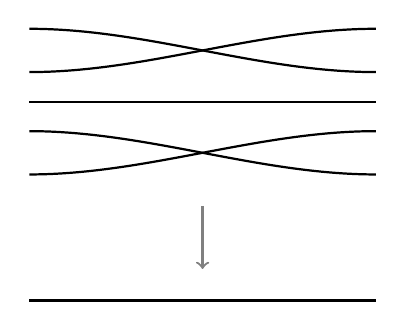
\begin{tikzpicture}[scale=1,line width=0.8pt]
  \draw (-2.2,1.60) .. controls (-0.7,1.60) and (0.7,1.05) .. (2.2,1.05);
  \draw (-2.2,1.05) .. controls (-0.7,1.05) and (0.7,1.60) .. (2.2,1.60);
  \draw (-2.2,0.675) -- (2.2,0.675);
  \draw (-2.2,0.30) .. controls (-0.7,0.30) and (0.7,-0.25) .. (2.2,-0.25);
  \draw (-2.2,-0.25) .. controls (-0.7,-0.25) and (0.7,0.30) .. (2.2,0.30);
  \draw[->,gray] (0,-0.65) -- (0,-1.45);
  \draw[line width=1.2pt] (-2.2,-1.85) -- (2.2,-1.85);
\end{tikzpicture}
\caption{\trBranchDivisor{}以重数 $2$ 出现的一个例子（见\mbox{练习~21.4.C}）。（依原书手绘图重绘。）}\label{fig:branch-divisor-multiplicity}
\end{figure}

作为对后文所见的一个动机，我们指出：在复几何中，从（复）曲线到曲线的非常值\trMap{}可以写在适当的局部坐标下，形如 $x\mapsto x^m=y$；由此我们看到 $\mathrm{d}y$ 拉回为 $mx^{m-1}\,\mathrm{d}x$，于是 $\Omega_{X/Y}$ 局部看起来就像「函数乘 $\mathrm{d}x$」模去 $mx^{m-1}\,\mathrm{d}x$ 的诸倍数。

现在考虑我们的\trMap{} $\pi\colon X\to Y$，取定 $p\in X$，并令 $q=\pi(p)$。由于 $\Omega$ 的构造对\trBaseChange{}表现良好（\mbox{定理~21.2.26(b)}），我们可以把 $Y$ 换成 $q$ 处局部环 $\OO_{Y,q}$ 的 $\Spec$；也就是说，我们可以假设 $Y=\Spec B$，其中 $B$ 是一个\trDVR（因为 $Y$ 是正则曲线），带有对应于 $q$ 的剩余域 $k=\bar{k}$。通过限制到 $X$ 中 $p$ 的一个仿射开邻域，我们假设 $X$ 也是仿射的。类似地，由于 $\Omega$ 的构造对\trLocalization{}表现良好（\mbox{练习~21.2.L}），我们可以把 $X$ 换成 $\Spec\OO_{X,p}$，从而假设 $X=\Spec A$，其中 $A$ 是一个\trDVR，而 $\pi$ 对应于 $B\to A$，并诱导剩余域的一个同构（仍有 $k=\bar{k}$）。

设它们的单值化元分别为 $s$ 与 $t$，满足 $t\mapsto us^n$，其中 $u$ 是 $A$ 的一个可逆元素。
\begin{tikzcd}
X\ar[d] & A & us^n \\
Y & B\ar[u] & t\ar[u,maps to]
\end{tikzcd}

回忆：一个\trDVR{}在 $k$ 上的诸\trDifferential{}由其单值化元的 $\mathrm{d}$ 生成（\mbox{练习~21.3.E}）。于是
\[
\mathrm{d}t=\mathrm{d}(us^n)=un\,s^{n-1}\,\mathrm{d}s+s^n\,\mathrm{d}u.
\]

这个 $\Spec A$ 上的\trDifferential{}消失的阶至少为 $n-1$；而当 $n$ 不被\trCharacteristic{}整除时，其阶恰为 $n-1$。若该阶为 $n-1$，我们称之为\textbf{\trTame\trRamification}（tame ramification）；若该阶更大，则称之为\textbf{\trWild\trRamification}（wild ramification）。我们把这一阶数加一，定义为 $X$ 的该点处的\textbf{\trRamificationIndex}（ramification index）。\footnote{原书此处作「to be the the ramification index」，衍一「the」，当为「the ramification index」之误，径改。——译者注}

\textbf{21.4.B.（练习）}\quad 证明：$\Omega_{X/Y}$ 在 $p\in X$ 处的次数恰是 $\pi$ 在 $p$ 处的分歧阶减 $1$。（曲线上\trCoherentSheaf{}的次数定义于 \S18.4.6。你将需要弄明白\trCoherentSheaf{}在一点处的\trLength{}是什么意思；例如参看\mbox{练习~6.5.M}。）

\textbf{21.4.C.（练习：以原像个数诠释\trRamificationDivisor）}\quad 在这道练习中，我们取基域 $k$ 为\trAlgClosedField。设 $q\in Y$ 之上的分歧全是\trTame\trRamification（在\trCharacteristic{} $0$ 时这总是成立）。证明：\trBranchDivisor{}在 $q$ 处的次数是 $\deg\pi-|\pi^{-1}(q)|$。于是，\trBranchDivisor{}的重数量度的正是：原像个数比次数少的程度（见\cref{fig:branch-divisor-multiplicity}）。

\textbf{21.4.3.\ \trhTheorem（\trRiemann--\trHurwitz{}公式）。}\ ——\ \emph{设 $\pi\colon X\to Y$ 是射影正则曲线之间的一个纯次数 $n$ 的有限可分\trMorphism。设 $R$ 为\trRamificationDivisor。那么}
\begin{equation*}\tag{21.4.3.1}\label{eq:riemann-hurwitz}
2g(X)-2=n(2g(Y)-2)+\deg R.
\end{equation*}

\textbf{21.4.D.（练习）}\quad 证明\trRiemann--\trHurwitz{}公式。提示：把「次数在正合列中可加」这一事实（\mbox{练习~18.4.I}）应用于 \eqref{eq:cotangent-left-exact}。回忆：线丛的次数在整射影曲线的有限态射之下拉回表现良好，见\mbox{练习~18.4.G}。既约曲线上的一支挠\trCoherentSheaf（比如 $\Omega_\pi$）的支撑在维数 $0$ 处（\mbox{练习~14.3.F(b)}），故 $\chi(\Omega_\pi)=\mathrm{h}^0(\Omega_\pi)$。证明：$R$ 作为除子的次数与其在 $\mathrm{h}^0$ 意义下的次数相同。

下面是\trRiemann--\trHurwitz{}公式的一些应用。

\textbf{21.4.4.}\ \emph{\trhExample{}。}\quad $R$ 的次数总为偶数：曲线的任何覆盖必定在偶数个点处分歧（以适当的重数计数）。

\textbf{21.4.E.（容易的练习）}\quad 证明：不存在从光滑射影既约\trGenus{} $2$ \trCurve{}到光滑射影既约\trGenus{} $3$ \trCurve{}的非常值\trMap{}。（提示：$\deg R\ge 0$。）

\textbf{21.4.5.}\ \emph{\trhDefinition{}。}\quad 若连通\trScheme{} $X$ 仅有的连通有限\trEtale{}覆盖是同构，我们就说 $X$ 是\textbf{在\trEtale{}拓扑下\trSimplyConnected}的（simply connected in the étale topology）。你看出来为什么「单连通」对这个概念是个合理的名字了吗？在下面这段简短的讨论之外，我们不会使用这个术语。

\textbf{21.4.6.}\ \emph{\trhExample{}（「$\mathbb{P}^1_k$ \trSimplyConnected」）。}\quad 若 $k=\bar{k}$，则 $\mathbb{P}^1_k$ 仅有的连通\trUnbranched{}的有限可分覆盖就是同构，理由如下。设 $X$ 连通，而 $X\to\mathbb{P}^1_k$ 无分歧。那么 $X$ 是一条曲线，并且由\mbox{练习~24.8.F(a)} 它正则。（这道练习虽在将来，你尽可以直接把这一点当作理所当然。这里不会有循环论证。）应用\trRiemann--\trHurwitz{}公式，并用\trRamificationDivisor{}为 $0$ 这一事实，我们得到 $2-2g_X=2d$，其中 $d\ge 1$、$g_X\ge 0$，由此得 $d=1$ 与 $g_X=0$。

\textbf{21.4.F.（练习：「\trCharacteristic{} $0$ 时 $\mathbb{A}^1_{\bar{k}}$ \trSimplyConnected」）}\quad 证明：若 $k=\bar{k}$ 的\trCharacteristic{}为 $0$，则 $\mathbb{A}^1_{\bar{k}}$ 仅有的连通\trUnbranched{}覆盖是它自身。（旁注：在\trCharacteristic{} $p$ 时这不必成立；$\Spec k[x,y]/(y^p-y-x)\to\Spec k[x]$ 就是这样一个\trMap，你自己便可证明。一旦代数基本群的理论得到发展，这句话就翻译为：「$\mathbb{A}^1$ 在\trCharacteristic{} $p$ 下不单连通」。这个覆盖是\textbf{\trArtin--\trSchreier{}覆盖}（Artin--Schreier cover）的一个例子。有趣的事实：群 $\mathbb{Z}/p$ 通过映射 $y\mapsto y+1$ 作用在这个覆盖上。这是一个\textbf{伽罗瓦覆盖}（Galois cover）的例子；你可以检验函数域的扩张是\trGalois{}的。）

\textbf{21.4.G.（不重要的练习）}\quad 推广\mbox{例~21.4.6} 与\mbox{练习~21.4.F}：去掉 $k=\bar{k}$ 的假设，并把「连通」改为「\trGeometricallyConnected」。

\textbf{21.4.7.}\ \emph{\trhExample{}：\trLuroth{}定理。}\quad 延续\mbox{定理~21.4.3} 的记号，设 $g(X)=0$。那么由\trRiemann--\trHurwitz{}公式 \eqref{eq:riemann-hurwitz}，$g(Y)=0$。（否则，若 $g(Y)$ 至少为 $1$，则\trRiemann--\trHurwitz{}公式的右边将会非负，从而不可能是左边的 $-2$。）不严格地说：从\trGenus{} $0$ \trCurve{}到正\trGenus{}曲线的\trMap{}只有常值\trMap。借助于曲线的覆盖与域扩张的认同（\mbox{定理~16.3.3}），这有一个并不显然的代数推论：$k(x)$ 的包含 $k$ 的子域都具有 $k(y)$ 的形式，其中 $y=f(x)$，而 $f\in k(x)$。

\begin{tikzcd}
k(x) & \mathbb{P}^1\ar[d] \\
K(C)\ar[ur,hook] & C & {=\mathbb{P}^1}
\end{tikzcd}

（结果表明，$\operatorname{char}k=0$ 与 $k=\bar{k}$ 这两个假设并不必要。）这就是\trLuroth{}定理。

\textbf{21.4.H.（练习）}\quad 用\trLuroth{}定理给\mbox{练习~7.5.K} 与\mbox{练习~7.5.M} 新的几何解法。（与那两道练习的提示中所建议的代数解法相比，这些论证不那么 ad hoc，而且更适合推广。）

\textbf{21.4.I.}\ \hard\ \textbf{（练习：\trGeometricGenus{}等于拓扑亏格）}\quad 这道练习是为具有一定复几何背景的读者准备的——他们知道\trRiemann--\trHurwitz{}公式在复解析范畴中成立。设 $C$ 是一条既约正则射影复曲线。证明：存在一个代数的非常值\trMap{} $\pi\colon C\to\mathbb{P}^1_{\mathbb{C}}$。请描述相应的\trRiemannSurface{}之间的\trMap。用\trRiemann--\trHurwitz{}公式证明：\trGenus{}的代数概念（用\trBranchedCover{} $\pi$ 计算）与\trGenus{}的拓扑概念（用同一个\trBranchedCover）相一致。（回忆：假设\mbox{奇迹~18.5.2}——即典范丛是\trSerre{}对偶化的——我们知道\trGeometricGenus{}等于算术亏格，见\mbox{练习~21.3.A}。）

\textbf{21.4.J.（不重要的练习）}\quad 设 $\pi\colon X\to Y$ 是正则曲线之间的一个\trDominant{}\trMorphism，而 $R$ 是 $\pi$ 的\trRamificationDivisor。证明：$\Omega_X(-R)\cong\pi^*\Omega_Y$。（这道练习在几何上令人愉悦，但我们用不到它。）提示：这句话说的是，我们可以把 $X$ 的开集 $\mathrm{U}$ 上的可逆层 $\pi^*\Omega_Y$ 诠释为恰是 $\mathrm{U}$ 上沿\trRamificationDivisor{}消失的那些\trDifferential。

\textbf{21.4.8.}\ \emph{非正式的例子：单变元 $d$ 次多项式的\trDiscriminant{}之次数。}\quad 你或许知道：存在一个次数为 $2d-2$ 的多项式，含于 $d$ 次多项式
\[
f(x)=a_dx^d+a_{d-1}x^{d-1}+\cdots+a_0=0
\]
的诸系数 $a_d,\dots,a_0$ 之中，它恰在 $f(x)$ 有重根时消失。例如当 $d=2$ 时，\trDiscriminant{}是 $a_1^2-4a_0a_2$。我们可以用\trRiemann--\trHurwitz{}公式如下地「算出」这个次数 $2d-2$。（下面这段非正式且不精确的讨论，请你努力把它弄明白。）为简单起见，我们在\trCharacteristic{} $0$ 的\trAlgClosedField{} $k$ 上工作。若取两个一般的 $d$ 次多项式 $g(x)$ 与 $h(x)$，则\trDiscriminant{}的次数「应当是」使得 $g(x)-\lambda h(x)$ 有二重根的那些 $\lambda\in k$ 的个数。考虑由 $x\mapsto[g(x),h(x)]$ 给出的态射 $\mathbb{P}^1\to\mathbb{P}^1$。（这里我们在源 $\mathbb{P}^1$ 上使用「仿射坐标」：$x$ 指的是 $[x,1]$。）那么这个态射的次数为 $d$。一个映到目标 $\mathbb{P}^1$ 中分支点 $[\lambda,1]$ 的分歧点 $a$，对应于 $a$ 是 $g(x)-\lambda h(x)$ 的二重根。于是分支点的个数应当就是所想要的\trDiscriminant{}的次数。由\trRiemann--\trHurwitz{}公式，共有 $2d-2$ 个分支点（诚然，是以重数计）。把这一论证变成一个证明是可能的，而且这样做很有意思。

\textbf{21.4.9.}\ \hard\ \textbf{曲线\trAutomorphismGroup{}的界。}\quad \trGenus{} $g\ge 2$ 的既约光滑射影曲线具有有限\trAutomorphismGroup，这是一个非平凡的事实。（$\mathbb{C}$ 上的证明见 [FK, \S5.1]。任意\trCharacteristic{}下的首个证明见 [Schm]，尽管如今已有更好的进路。）姑且承认这一事实，我们便能证明：在\trCharacteristic{} $0$ 时，\trAutomorphismGroup{}的阶至多为 $84(g-1)$（\emph{\trHurwitz{}自同构定理}（Hurwitz's Automorphisms Theorem）），做法如下。

设 $C$ 是\trAlgClosedField{} $k=\bar{k}$（\trCharacteristic{} $0$）上一条\trGenus{} $g\ge 2$ 的既约光滑射影\trCurve。设 $G$ 是 $C$ 的\trAutomorphism{}的一个\emph{有限}\trGroup。我们现在证明 $|G|\le 84(g-1)$。（$k$ 不代数闭的情形，经基变换到 $\bar{k}$ 后即可迅速打发。）

\textbf{21.4.K.（练习）}\quad
（a）设 $C'$ 是对应于 $k$ 上的域扩张 $K(C)^G$ 的那条光滑射影曲线（经\mbox{定理~16.3.3}）。（$K(C)^G$ 指 $K(C)$ 的 $G$-不变元。）描述一个次数为 $|G|$ 的态射 $\pi\colon C\to C'$，以及 $C$ 上一个与 $\pi$ 交换的\trFaithful{} $G$-作用。
（b）证明：在 $\pi$ 的每个分支点之上，诸原像全都以相同的阶分歧（因为 $G$ 在其上传递地作用）。设共有 $n$ 个分支点，而第 $i$ 个的分歧为 $r_i$（每个都出现 $|G|/r_i$ 次）。
（c）用\trRiemann--\trHurwitz{}公式证明
\[
(2g-2)=|G|\biggl(2g(C')-2+\sum_{i=1}^{n}\frac{r_i-1}{r_i}\biggr).
\]

为使 $|G|$ 最大，我们希望使
\begin{equation*}\tag{21.4.9.1}\label{eq:hurwitz-automorphism-minimize}
2g(C')-2+\sum_{i=1}^{n}\frac{r_i-1}{r_i}
\end{equation*}
在 \eqref{eq:hurwitz-automorphism-minimize} 为正的约束下最小。注意 $1/42$ 是可以取到的：取 $g(C')=0$、$n=3$、$(r_1,r_2,r_3)=(2,3,7)$。

\textbf{21.4.L.（练习）}\quad 通过分别考虑下列诸情形，证明你无法做得比 $1/42$ 更好：
（a）$g(C')>1$；
（b）$g(C')=1$；
（c）$g(C')=0$ 且 $n\ge 5$；
（d）$g(C')=0$ 且 $n=4$；以及
（e）$g(C')=0$ 且 $n=3$。

\textbf{21.4.M.（练习）}\quad 用 \eqref{eq:hurwitz-automorphism-minimize} 至少为 $1/42$ 这一事实证明该结果。

\textbf{21.4.10.}\ \emph{\trhRemark{}。}\quad 在正\trCharacteristic{}中，自同构可以多得多。例如 [Stic]：在\trCharacteristic{} $p$ 时，若 $p^n$ 是一个不为 $2$ 的素数幂，则仿射曲线 $y^{p^n}=x+x^{p^n+1}$ 的完备化（「紧化」\footnote{原书此处作「compacitification」，当为「compactification」之误，径改。——译者注}）具有\trGenus{} $g=p^n(p^n-1)/2$，而其\trAutomorphismGroup{}的阶为 $p^{3n}(p^{3n}+1)(p^{2n}-1)$。


\section{借余切丛理解光滑簇}

本节中，我们将构造代数闭域上的簇的一些双有理不变量（例如\trGeometricGenus），为\trUnramified{}态射这一观念提供动机，证明簇「几乎处处光滑」，并初窥\trHodge{}理论。

\textbf{21.5.1. \trGeometricGenus{}与其他源自 $i$-形式的双有理不变量。}\quad 设 $X$ 是 $k$ 上的射影\trScheme。那么 $\mathrm{h}^0(X,\Omega_{X/k})$ 是 $X$ 的一个不变量。事实上，如下面的\mbox{练习~21.5.A} 所示，当 $X$ 光滑时，它与相关的一些不变量都是\emph{双有理不变量}。我们先定义\textbf{（相对）$i$-形式层}（sheaf of (relative) $i$-forms）%
$\Omega^i_{X/Y}:=\wedge^i\Omega_{X/Y}$。$\Omega^i_{X/Y}$ 的\trSection（在某个\trOpenSet{}上）称为\textbf{（相对）$i$-形式}（在该\trOpenSet{}上）。

\textbf{21.5.2.}\ \emph{笑话。}\quad 老麦当劳有一个形式；$e_i\wedge e_i=0$。%
\footnote{译注：此句戏仿英文童谣《老麦当劳有个农场》（\emph{Old MacDonald Had a Farm}）中的唱词「Old MacDonald had a farm, E--I--E--I--O」，原文「had a form; $e_i\wedge e_i=0$」与之谐音。}

\textbf{21.5.A.（练习：$\mathrm{h}^0(X,\Omega^i_{X/k})$ 是双有理不变量）}\quad 设 $X$ 与 $X'$ 是彼此双有理等价的不可约光滑射影 $k$-\trVariety。证明（对每个 $i$）：$\mathrm{H}^0(X,\Omega^i_{X/k})\cong\mathrm{H}^0(X',\Omega^i_{X'/k})$。（提示：取定双有理映射 $\phi\colon X\dashrightarrow X'$。由\mbox{练习~15.3.B}，$\phi$ 的\trDomainOfDefinition{} $U$ 的\trComplement{}余维数至少为 $2$。把诸 $i$-形式从 $X'$ 拉回到 $U$ 上，我们便得到一个映射 $\phi^*\colon\mathrm{H}^0(X',\Omega^i_{X'/k})\to\mathrm{H}^0(U,\Omega^i_{X/k})$。利用\mbox{\trAlgebraic\trHartogs{}引理~13.5.19} 以及 $\Omega^i$ 是\trLocallyFreeSheaf{}这一事实，证明该映射可以延拓为映射 $\phi^*\colon\mathrm{H}^0(X',\Omega^i_{X'/k})\to\mathrm{H}^0(X,\Omega^i_{X/k})$。若 $\psi\colon X'\dashrightarrow X$ 是逆有理映射，我们同样得到一个映射 $\psi^*\colon\mathrm{H}^0(X,\Omega^i_{X/k})\to\mathrm{H}^0(X',\Omega^i_{X'/k})$。证明 $\phi^*$ 与 $\psi^*$ 互为逆映射，办法是证明每个复合映射都在 $X$ 或 $X'$ 的某个稠密\trOpenSubset{}上为恒等。）

\textbf{21.5.3.}\ \emph{典范丛 $\mathscr{K}_X$ 与\trGeometricGenus{} $\mathrm{p}_g(X)$。}\quad 若 $X$ 是 $n$ 维光滑 $k$-簇，则可逆层（即\trLineBundle）$\det\Omega_{X/k}=\Omega^n_{X/k}$（「\trAlgebraicVolumeForm」层）具有特殊的重要性，它被称为\textbf{典范（可逆）层}，或者\textbf{典范（线）丛}，记作 $\mathscr{K}_X$（或 $\mathscr{K}_{X/k}$）。如 \S18.5.2 所述，若 $X$ 是射影的，则 $\mathscr{K}_X$ 就是\trSerreDuality{}的陈述中出现的那个\trCanonical{}层 $\omega_X$；这一点我们将在 \S29.4 中予以建立（见\mbox{\trDesideratum{}~29.1.1}）。

\textbf{21.5.B.（练习：$\mathscr{K}_X$ 的伴随公式）}\quad 设 $X$ 是光滑簇，$Z$ 是 $X$ 的一个光滑子簇。证明
\[
\mathscr{K}_Z\cong\mathscr{K}_X|_Z\otimes\det\mathscr{N}_{Z/X}.
\]
（提示：将\mbox{练习~14.2.P} 应用于\mbox{定理~21.2.31}。）特别地，由\mbox{练习~21.2.J}，若 $Z$ 的余维数为 $1$，则
\[
\mathscr{K}_Z\cong(\mathscr{K}_X\otimes\OO_X(Z))|_Z,
\]
这个式子更常用、也更紧凑的写法是 $\mathscr{K}_X(Z)|_Z$。伴随公式常被归纳地用于完全相交的情形；\mbox{练习~21.5.G} 即是一例。（伴随公式的其他版本见\mbox{练习~20.2.B(a)} 与 \S29.4。）

\textbf{21.5.4.}\ \emph{\trhDefinition。}\quad 若 $X$ 是射影（甚至是固有）的光滑 $k$-簇，则双有理不变量 $\mathrm{h}^0(X,\mathscr{K}_X)=\mathrm{h}^0(X,\Omega^n_{X/k})$ 具有特殊的重要性。它被称为\textbf{\trGeometricGenus}，记作 $\mathrm{p}_g(X)$。曲线的情形已在 \S21.3.1 中见过。若 $X$ 是一个未必光滑或射影的不可约簇，则「\trGeometricGenus」一词指的是与 $X$ 双有理等价的某个光滑射影簇 $X'$ 的 $\mathrm{h}^0(X',\mathscr{K}_{X'})$。（由\mbox{练习~21.5.A}，这与 $X'$ 的选取无关。）例如，若 $X$ 是 $k$ 上的一条既约不可约射影\trCurve，则\trGeometricGenus{}就是 $X$ 的\trNormalization{}的\trGenus。（但在更高的维数，这样的 $X'$ 是否存在并不清楚。一件非平凡的事实是：在\trCharacteristic{} $0$ 时这的确成立，而在正\trCharacteristic{}时这还是未知的；见\mbox{注记~22.4.6}。）

堪称奇迹的是：对一条复曲线而言，\trGeometricGenus{}与\trTopologicalGenus{}及\trArithmeticGenus{}相同。\mbox{练习~18.5.A} 证明了\trGeometricGenus{}与算术亏格相等（假定\mbox{奇迹~18.5.2}，即典范丛是\trSerre{}对偶化的）。我们马上就会在关于\trRiemann--\trHurwitz{}公式的讨论中把\trGeometricGenus{}与拓扑亏格联系起来（\mbox{练习~21.4.I}）。

\textbf{21.5.C.（练习）}\quad 设 $Z$ 是 $\mathbb{P}^3_{\bar{k}}$ 中一张次数为 $d$ 的正则曲面。计算 $Z$ 的\trGeometricGenus{} $\mathrm{p}_g(Z)$。证明 $\mathbb{P}^3_{\bar{k}}$ 中不存在有理的正则四次曲面（即与 $\mathbb{P}^2_{\bar{k}}$ 双有理等价，\mbox{定义~7.5.5}）。（这样的四次曲面是 K3 \emph{曲面}的一些例子；见\mbox{练习~21.5.I}。）

\textbf{21.5.5. 簇的几类重要类型：Fano、Calabi--Yau、一般型。}\quad 设 $X$ 是光滑射影 $k$-簇。若 $\mathscr{K}_X^\vee$ 是\trAmple{}的，则称 $X$ 是 \textbf{Fano} 的；若 $\mathscr{K}_X\cong\OO_X$，则称 $X$ 是 \textbf{Calabi--Yau} 的。（警示：Calabi--Yau 还有别的定义。）

\textbf{21.5.D.（练习）}\quad 对一切 $j\ge 0$，光滑射影 $k$-簇的\textbf{第 $j$ 个多亏格}（jth plurigenus）是 $\mathrm{h}^0(X,\mathscr{K}_X^{\otimes j})$。证明第 $j$ 个多亏格是双有理不变量。

（相比之下，当 $j<0$ 时 $\mathrm{h}^0(X,\mathscr{K}^{\otimes j})$ 不是双有理不变量。例如，你可以证明：对 $X=\mathbb{P}^2_k$ 与 $X=\mathrm{Bl}_p\mathbb{P}^2_k$ 而言，$\mathrm{h}^0(X,\mathscr{K}^{\vee})$ 的值有所不同。）

$X$ 的\textbf{\trKodaira{}维数}（Kodaira dimension），记作 $\kappa(X)$，追踪的是诸个多亏格的增长速率。它是使 $\mathrm{h}^0(X,\mathscr{K}_X^{\otimes j})/j^k$ 有界（当 $j$ 遍历正整数时）的最小的 $k$；唯一的例外是：若诸个多亏格 $\mathrm{h}^0(X,\mathscr{K}_X^{\otimes j})$ 全为 $0$，则我们说 $\kappa(X)=-1$。小平维数「总是存在」，并且它是诸第 $j$ 个「多典范有理映射」（pluricanonical rational maps）的像的维数中的最大者——这是一件非平凡的事实。后一事实蕴涵：小平维数是介于 $-1$ 与 $\dim X$ 之间（含两端）的整数。\mbox{练习~21.5.D} 表明小平维数是双有理不变量。若 $\kappa(X)=\dim X$，我们说 $X$ 是\textbf{一般型}（general type）的。（关于小平维数的更多信息，见 [Ii, \S10.5]。）

\textbf{21.5.E.（练习）}\quad 证明：若 $\mathscr{K}_X$ 是\trAmple{}的，则 $X$ 是一般型的。

\textbf{21.5.F.（练习）}\quad 证明：（域 $k$ 上的）光滑\trGeometricallyIrreducible{}射影\trCurve{}当其\trGenus{}为 $0$（相应地，$1$，大于 $1$）时是 Fano（相应地，Calabi--Yau，一般型）的。

\mbox{练习~21.5.F} 的「三分法」（trichotomy）在精神实质上正是如下现象的原因：曲线的行为依其所属的三个类而各不相同（见 \S19.6.1）。在某种意义上，这一三分法的一些重要侧面可以延伸到更高的维数，这也是我们要作这些定义的部分理由。现在我们在完全相交的情形探究这一三分法。

\textbf{21.5.G.（练习）}\quad 设 $X$ 是 $\mathbb{P}^N_k$ 中由次数为 $d_1,\dots,d_n$ 的超曲面给出的光滑完全相交，其中 $k$ 是代数闭的。
（a）证明 $\mathscr{K}_X\cong\OO(-N-1+d_1+\cdots+d_n)|_X$。
（b）证明：若 $-N-1+d_1+\cdots+d_n$ 为负（相应地，为零，为正），则 $X$ 是 Fano（相应地，Calabi--Yau，一般型）的。
（c）找出 $N$ 与 $d_1,\dots,d_n$ 的所有可能的取值，使得 $X$ 是维数至多为 $3$ 的 Calabi--Yau。留意这张清单有多小。

\textbf{21.5.H.（容易的练习）}\quad 光滑 Fano 曲面称为\textbf{\trDelPezzo{}曲面}（del Pezzo surface）（它是曲面的\trEnriques--\trKodaira{}分类的一部分）。证明下列曲面都是 del Pezzo 曲面：(a) $\mathbb{P}^2_k$；(b) $\mathbb{P}^1_k\times\mathbb{P}^1_k$；(c) $\mathbb{P}^3_k$ 中次数至多为 $3$ 的光滑曲面。（这张清单有一些冗余！del Pezzo 曲面的其余例子在\mbox{注记~27.3.7} 中有描述；其中的一个早在 \S19.8.3 中就已出现过。）

\textbf{21.5.I.（练习）}\quad 域 $k$ 上的一个 \textbf{K3 曲面}（K3 surface）是 $k$ 上一个固有、光滑、\trGeometricallyConnected{}的 Calabi--Yau 曲面 $X$，满足 $\mathrm{H}^1(X,\OO_X)=0$。（\trWeil{}曾写道：K3 曲面的命名是为了纪念\trKummer、\trKahler、\trKodaira{}三位数学家以及 K2 山峰，[BPV, p.~288]。）证明\mbox{练习~21.5.G(c)} 中维数为 $2$ 的（光滑）Calabi--Yau 完全相交都是 K3 曲面。

\textbf{21.5.6.}\ \emph{诱人的题外注记。}\quad 若你把切出完全相交 K3 曲面的那些超曲面的次数（见\mbox{练习~21.5.G(c)}），与切出完全相交典范曲线的超曲面的次数（见 \S19.8.2 与\mbox{练习~19.8.E}）作个比较，你会注意到一个引人注目的巧合。当然，这根本不是巧合。

\textbf{21.5.J.（练习：并非一切都能纳入这一三分法）}\quad 设 $C$ 是\trGenus{}大于 $1$ 的光滑射影不可约复曲线。证明 $C\times_\mathbb{C}\mathbb{P}^1_\mathbb{C}$ 既不是 Fano 的，也不是 Calabi--Yau 的，还不是一般型的。（提示：\mbox{练习~21.2.U}。）

\textbf{21.5.7.}\ \hard\ \textbf{\trKodaira{}消失。}\quad \trKodaira{}消失定理是代数几何中好几个领域的重要工具。我们出于文化修养的缘故陈述它，但不予证明（因此也不会用到它）。

\textbf{21.5.8.\ \trhTheorem（\trKodaira{}消失定理）。}\ ——\ \emph{设 $k$ 是\trCharacteristic{} $0$ 的域，而 $X$ 是光滑射影 $k$-簇。那么对任意\trAmple{}\trInvertibleSheaf{} $\mathscr{L}$，当 $i>0$ 时 $\mathrm{H}^i(X,\mathscr{K}_X\otimes\mathscr{L})=0$。}

\textbf{21.5.9.}\quad 对\trCharacteristic{}的限制是必要的：\trRaynaud{}给出了一个在正\trCharacteristic{}下小平消失失效的例子 [Ra]。原始证明的做法是：先证复解析的版本，再借\trSerre{}的 GAGA 定理 [Se3] 把它转移成一个复的代数陈述。一般的\trCharacteristic{} $0$ 情形可以归结为 $\mathbb{C}$ 的情形——任何这类归结常常被（有些含糊地）称作\trLefschetz{}原理（Lefschetz principle）的一次应用。（\trLefschetz{}原理的一个精确表述，连同适用于任意\trCharacteristic{}的短证明，见 [Ek]；一个推广见 [FR]；更多背景见 [MO90551]。）\trRaynaud{}后来给出了小平消失的一个戏剧性的代数证明，其中\emph{用到}了正\trCharacteristic（！）；见 [De1] 或 [Il]。

\textbf{21.5.K.（练习）}\quad 在 $\dim X=1$ 的情形以及对 $\mathbb{P}^n_k$ 证明小平消失定理。（这两种情形都不需要\trCharacteristic{} $0$ 的假设。）

\textbf{21.5.10.}\ \hard\ \textbf{初窥\trHodge{}理论。}\quad 不变量 $\mathrm{h}^j(X,\Omega^i_{X/k})$ 称为 \textbf{\trHodge{}数}（Hodge number）$\mathrm{h}^{i,j}(X)$。由\mbox{练习~21.5.A}，诸 $\mathrm{h}^{i,0}$ 是双有理不变量。我们很快就会看到（在\mbox{练习~21.5.O} 中），这一点并非对所有的 $\mathrm{h}^{i,j}$ 都成立。

\textbf{21.5.L.（练习）}\quad 设 $X$ 是光滑射影簇。假定\mbox{奇迹~18.5.2}（典范丛是\trSerre{}对偶化的），证明诸\trHodge{}数满足对称性 $\mathrm{h}^{p,q}=\mathrm{h}^{n-p,n-q}$。（\mbox{练习~14.2.O} 会派上用场。）

\textbf{21.5.M.（练习：射影空间的 \trHodge{}数）}\quad 证明：当 $0\le p=q\le n$ 时 $\mathrm{h}^{p,q}(\mathbb{P}^n_k)=1$，否则 $\mathrm{h}^{p,q}(\mathbb{P}^n_k)=0$。（提示：使用欧拉正合列（\mbox{定理~21.3.6}），并应用\mbox{练习~14.2.N}。）

\textbf{21.5.11.}\ \emph{\trhRemark{}：\trHodge{}菱形。}\quad 在 $k=\mathbb{C}$ 上，还会发生更多的奇迹。若 $X$ 是不可约光滑射影复簇，那么结果表明存在一个直和分解
\begin{equation*}\tag{21.5.11.1}\label{eq:hodge-decomposition}
\mathrm{H}^m(X,\mathbb{C})=\bigoplus_{i+j=m}\mathrm{H}^j(X,\Omega^i_{X/\mathbb{C}}),
\end{equation*}
从而 $\mathrm{h}^m(X,\mathbb{C})=\sum_{i+j=m}\mathrm{h}^{i,j}$，于是诸\trHodge{}数（纯代数的对象）给出了贝蒂数（Betti numbers；先验地看，这是拓扑信息）。此外，复共轭把 $\mathrm{H}^j(X,\Omega^i_{X/\mathbb{C}})$ 与 $\mathrm{H}^i(X,\Omega^j_{X/\mathbb{C}})$ 互换，由此得到
\begin{equation*}\tag{21.5.11.2}\label{eq:hodge-symmetry}
\mathrm{h}^{i,j}=\mathrm{h}^{j,i}.
\end{equation*}
（题外话：这条附加的对称性在\trCharacteristic{} $0$ 下普遍成立，但在正\trCharacteristic{}下可能失效；例如见 [Ig, p.~966]、[Mu1, \S III]、[Se4, Prop.~16]。）这是广阔而丰富的\trHodge{}理论这一主题的开端（想多知道一点，见 [GH1, \S0.6]；想多知道很多，见 [Vo]）。

若我们把诸\trHodge{}数写成一个菱形，其中 $\mathrm{h}^{i,j}$ 是第 $i+j$ 行内的第 $i$ 个条目，那么这个菱形便具有分别来自\trSerreDuality{}与复共轭的两个对称性。例如，一个不可约光滑射影复曲面的\trHodge{}菱形将具有如下形状：
\[
\begin{array}{ccccc}
 & & 1 & & \\
 & q & & q & \\
 \mathrm{p}_g & & \mathrm{h}^{1,1} & & \mathrm{p}_g \\
 & q & & q & \\
 & & 1 & &
\end{array}
\]
其中 $\mathrm{p}_g$ 是该曲面的\trGeometricGenus，而 $q=\mathrm{h}^{0,1}=\mathrm{h}^{1,0}=\mathrm{h}^{2,1}=\mathrm{h}^{1,2}$ 称为该曲面的\textbf{不规则性}（irregularity）。再举一例，由\mbox{练习~21.5.M}，$\mathbb{P}^n$ 的\trHodge{}菱形除竖直对称轴上的一列 $1$ 之外全为 $0$。

你不需要那两条未加证明的陈述 \eqref{eq:hodge-decomposition} 或 \eqref{eq:hodge-symmetry}，也能解出下面的习题。

\textbf{21.5.N.（练习）}\quad 假定\mbox{奇迹~18.5.2}（典范丛是\trSerre{}对偶化的），证明：域 $k$ 上一条光滑射影\trGeometricallyIrreducible{}、亏格为 $g$ 的曲线，其\trHodge{}菱形如下：
\[
\begin{array}{ccc}
 & 1 & \\
 g & & g \\
 & 1 &
\end{array}
\]

\textbf{21.5.O.（练习）}\quad 证明 $\mathbb{P}^1_k\times\mathbb{P}^1_k$ 的\trHodge{}菱形如下：
\[
\begin{array}{ccccc}
 & & 1 & & \\
 & 0 & & 0 & \\
 0 & & 2 & & 0 \\
 & 0 & & 0 & \\
 & & 1 & &
\end{array}
\]
把你得到的答案与 $\mathbb{P}^2_k$ 的\trHodge{}菱形（\mbox{练习~21.5.M}）作比较，证明 $\mathrm{h}^{1,1}$ 不是双有理不变量。

注意在上述两种情形中，$\mathrm{h}^{1,1}$ 都是\trPicard{}数 $\rho$（定义见 \S18.4.12）。一般地，$\rho\le\mathrm{h}^{1,1}$（\trCharacteristic{} $0$ 时见 [GH1, \S3.5, pp.~456--7]）。

\textbf{21.5.12.}\ \hard\ \textbf{题外：无穷小形变与自同构。}\quad 把这件事说精确超出了本书的范围，但若 $X$ 是一个簇，则 $\mathrm{H}^0(X,\mathscr{T}_X)$ 参数化 $X$ 的无穷小自同构，而 $\mathrm{H}^1(X,\mathscr{T}_X)$ 参数化 $X$ 的无穷小形变。作为一个例子，若 $X=\mathbb{P}^1$（在某个域上），则 $\mathscr{T}_{\mathbb{P}^1}\cong\OO(2)$（\S21.3.2），于是 $\mathrm{h}^0(\mathbb{P}^1,\mathscr{T}_{\mathbb{P}^1})=3$，而这恰好就是 $\mathbb{P}^1$ 的自同构群的维数（\mbox{练习~15.5.A}）。

\textbf{21.5.P.（练习）}\quad 用欧拉正合列（\mbox{定理~21.3.6}）计算 $\mathrm{h}^0(\mathbb{P}^n_k,\mathscr{T}_{\mathbb{P}^n_k})$，并将此与 $\mathbb{P}^n_k$ 的自同构群的维数（\mbox{练习~15.5.A}）作比较。

\textbf{21.5.Q.（练习）}\quad 证明 $\mathrm{H}^1(\mathbb{P}^n_A,\mathscr{T}_{\mathbb{P}^n_A})=0$。（于是射影空间不能形变，是「刚性」的。）

\textbf{21.5.R.（练习）}\quad 假定\mbox{奇迹~18.5.2}（典范丛是\trSerre{}对偶化的），对 $k$ 上一条亏格为 $g$ 的光滑射影\trGeometricallyIrreducible{}曲线 $C$，就 $i=0$ 与 $1$ 计算 $\mathrm{h}^i(C,\mathscr{T}_C)$。你应当注意到：亏格为 $0$、$1$ 与 $g>1$ 时，$\mathrm{h}^i(C,\mathscr{T}_C)$ 分别为 $0$、$1$ 与 $3g-3$；做完之后，重读 \S19.8.4。


\section{一般光滑性及其推论}

现在，我们能够证实一件你或许早已凭直觉感到的事情。在正\trCharacteristic{}时，这是一条困难的定理，因为它用到了交换代数中一个我们未曾证明的结果。

\textbf{21.6.1.\ \trhTheorem（\trVariety{}的一般光滑性）。}\ ——\ \emph{设 $X$ 是\trPerfectField{} $k$ 上一个\trIntegral{}的\trFiniteType{} $k$-\trScheme，维数为 $n$，那么存在 $X$ 的一个\trDense\trOpenSubset{} $\mathrm{U}$，使得 $\mathrm{U}$（在 $k$ 上）是\trSmooth{}的，且维数为 $n$。}

于是，由\mbox{练习~13.2.R} 结合\mbox{事实~13.8.2}（\trRegular{}的\trLocalization{}是\trRegular{}的），$\mathrm{U}$ 是\trRegular{}的。\mbox{定理~21.6.4} 将把这一结果推广到\trSmooth\trMorphisms，代价是须限制在\trCharacteristic{} $0$ 之中。

若 $k$ 不完全时会出什么问题，可在 \S13.2.9 中找到一个例子。

\emph{证明。}\ $n=0$ 的情形是显然的，故我们设 $n>0$。

我们将证明在\trGenericPoint{}处秩为 $n$。那么，由\trCoherentSheaf{}之秩的\trUpperSemicontinuous{}性（\mbox{练习~14.3.J}），在\trGenericPoint{}的某个\trOpen\trNeighborhood{}内秩必为 $n$，证明便告完成。

于是我们还须验证的是：若 $K$ 是一个维数为 $n$ 的\trIntegral{}的\trFiniteType{} $k$-\trScheme{}的\trFractionField，也就是说（由\mbox{定理~12.2.1}），若 $K/k$ 是一个\trTrDeg{}为 $n$ 的\trFieldExtension，那么 $\Omega_{K/k}$ 是一个 $n$ 维\trVectorSpace。但\trPerfectField{}的每个\trFinitelyGenerated{}扩张都是\trSeparablyGenerated{}的（\mbox{定理~10.5.17}），于是结论由\mbox{练习~21.2.M(b)} 得出。\hfill$\square$

\textbf{21.6.2.\ \mbox{定理~13.8.3} 的证明：\trRegular\trLocalRing{}的\trLocalization{}仍是\trRegular{}的——完全域上\trVariety{}的情形。}\quad \mbox{定理~21.6.1} 使我们得以证明\mbox{定理~13.8.3}（\mbox{事实~13.8.2} 的一个重要情形）。

设 $Y$ 是\trPerfectField{} $k$ 上的一个\trVariety，并在其诸\trClosedPoint{}处\trRegular（于是由\mbox{练习~13.2.R}，$Y$ 是\trSmooth{}的），又设 $\eta$ 是 $Y$ 的一点。我们将证明 $Y$ 在 $\eta$ 处\trRegular。令 $X=\overline{\eta}$。由\mbox{定理~21.6.1}，$X$ 含有一个由\trSmooth{}点组成的\trDense{}（＝非空）\trOpenSubset。把 $X$ 位于该\trOpenSubset{}之外的点丢弃、从而缩小 $Y$ 之后，我们便可假定 $X$ 是\trSmooth{}的。

那么，\mbox{定理~21.2.31}（\trSmooth\trVariety{}的余正规正合列的正合性）蕴涵：$\mathscr{I}/\mathscr{I}^2$ 是一个秩为 $\operatorname{codim}_{X/Y}=\dim\OO_{Y,\eta}$ 的\trLocallyFreeSheaf。

\textbf{21.6.A.（练习）}\quad 设 $\mathfrak{m}$ 是 $\OO_{Y,\eta}$ 的\trMaximalIdeal。把 $\mathscr{I}/\mathscr{I}^2$ 在 $X$ 的\trGenericPoint{} $\eta$ 处的\trStalk{}与 $\mathfrak{m}/\mathfrak{m}^2$ 等同起来。由此完成\mbox{定理~13.8.3} 的证明。\hfill$\square$

\textbf{21.6.B.（棘手练习：\trVariety{}的\trRegular\trLocalRing{}的\trLocalization{}仍是\trRegular{}的——\mbox{定理~13.8.3} 之后所许诺者）}\quad 设 $(A,\mathfrak{m})$ 是一个\trRegular\trLocalRing，同时它是一个\trFinitelyGenerated{} $k$-代数的\trLocalization，其中 $k$ 是完全域。证明：$A$ 在任一\trPrimeIdeal{}处的\trLocalization{}仍是一个\trRegular\trLocalRing。

\textbf{21.6.3.\ \trMorphisms{}的一般光滑性与\trKleiman--\trBertini{}定理。}\quad 现在我们来讨论若干重要的结果，它们都归于「\trMorphisms{}的一般光滑性」这一名目之下。所有这些都要求在\trCharacteristic{} $0$ 中工作。

\textbf{21.6.4.\ \trhTheorem（源上的一般光滑性）。}\ ——\ \emph{(a) 设 $\pi\colon X\to Y$ 是\trIntegral{}的\trNoetherian{}\trScheme{}之间的一个\trDominant\trFiniteType{}\trMorphism，使得 $\operatorname{char}K(Y)$（$=\operatorname{char}K(X)$）为零。那么存在一个非空（＝\trDense）的\trOpenSet{} $\mathrm{U}\subset X$，使得 $\pi|_{\mathrm{U}}$ 是\trSmooth{}的，相对维数为 $\operatorname{trdeg}K(X)/K(Y)$。}

\emph{(b) 设 $k$ 是\trCharacteristic{} $0$ 的域，而 $\pi\colon X\to Y$ 是\trIntegral{}的 $k$-\trVariety{}之间的一个\trDominant\trMorphism。那么存在一个非空（＝\trDense）的\trOpenSet{} $\mathrm{U}\subset X$，使得 $\pi|_{\mathrm{U}}$ 是\trSmooth{}的，相对维数为 $\dim X-\dim Y$。}

\textbf{21.6.C.（练习：\mbox{练习~12.2.D} 中所许诺）}\quad 设 $f_1,\dots,f_n\in k[x_1,\dots,x_n]$，其中 $k$ 是\trCharacteristic{} $0$ 的域。证明：诸 $f_1,\dots,f_n$ \trAlgebraicallyDependent，当且仅当\trJacobianMatrix{}的\trDeterminant{}恒为零。提示：为什么这个练习恰好被安排在\mbox{定理~21.6.4} 之后给出？

\textbf{21.6.5.\ \trhExample。}\quad \mbox{定理~21.6.4} 在正\trCharacteristic{}时失效：考虑\trPurelyInseparable{}扩张 $\mathbb{F}_p(t)/\mathbb{F}_p(t^p)$。同样的问题甚至可能在\trCharacteristic{} $p$ 的\trAlgClosedField{}上出现：考虑 $\mathbb{A}^1_k=\Spec k[t]\to\Spec k[u]=\mathbb{A}^1_k$，由 $u\mapsto t^p$ 给出。%
\footnote{原书此处作「$\mathbb{A}^1_{k'}$」，当为「$\mathbb{A}^1_k$」之误——该态射即 $\Spec k[t]\to\Spec k[u]$，两端同在 $k$ 上——径改。——译者注}

\emph{证明。}\ 令 $n=\operatorname{trdeg}K(X)/K(Y)$。我们可以把 $Y$ 换成一个\trAffine\trOpenSubset{} $\Spec B$，再把 $X$ 换成一个\trAffine\trOpenSubset{} $\Spec A$，于是 $\pi$ 就对应于\trRingMorphism{} $B\to A$。选取 $n$ 个元素 $x_1,\dots,x_n\in A$，使它们构成 $K(A)/K(B)$ 的一组\trTranscendenceBase。（你看出为什么可以选取它们落在 $A$ 中吗？）再选取一些附加的元素 $x_{n+1},\dots,x_N\in A$，使得 $x_1,\dots,x_N$ 把 $A$ 生成为一个 $B$-代数。

对 $i=0,\dots,n$，令 $F_i$ 为 $K(A)$ 在 $K(B)$ 上由 $x_1,\dots,x_i$ 生成的子域。例如，$F_0=K(B)$，$F_N=K(A)$，而当 $i\le n$ 时，$F_i/K(B)$ 是\trPurelyTranscendental\trFieldExtension。对 $i=n+1,\dots,N$，$x_i\in K(A)$ 在 $F_{i-1}$ 上的\trMinimalPolynomial（$F_{i-1}[t]$ 中的一个元素）可以解读为 $\mathfrak{m}_i(x_1,\dots,x_{i-1},t)$ 的形式，其中 $\mathfrak{m}_i\in K(B)[y_1,\dots,y_{i-1},t]$。把 $\mathfrak{m}_i$ 乘以其诸系数分母之乘积，我们便得到 $M_i\in B[y_1,\dots,y_{i-1},t]$，使得 $M_i(x_1,\dots,x_{i-1},t)\in F_{i-1}[t]$ 也是 $x_i\in K(A)$ 在 $F_{i-1}$ 上的\trMinimalPolynomial。于是
\begin{equation*}
K(A)=K(B)(x_1,\dots,x_n)[y_{n+1},\dots,y_N]/I,
\tag{21.6.5.1}\label{eq:generic-smoothness-field}
\end{equation*}
其中
\[
\begin{aligned}
I=\bigl(&M_{n+1}(x_1,\dots,x_n,y_{n+1}),\ M_{n+2}(x_1,\dots,x_n,y_{n+1},y_{n+2}),\\
&\dots,\ M_N(x_1,\dots,x_n,y_{n+1},\dots,y_N)\bigr).
\end{aligned}
\]
定义 $A':=B[y_1,\dots,y_N]/(M_{n+1}(y_1,\dots,y_{n+1}),\dots,M_N(y_1,\dots,y_N))$。

令 $X':=\Spec A'$。设 $Z_1,\dots,Z_s$ 是 $X'$ 的诸\trIrreducibleComponent。（由 $B$ 的诺特性，它们只有有限多个：\mbox{练习~3.6.T} 与\mbox{命题~3.6.15}。）

它们当中恰有一个——比如说 $Z=Z_1$——\trDominant{} $\Spec B$（因为由 \eqref{eq:generic-smoothness-field}，$A'\otimes_B K(B)\cong K(A)$）。令 $\mathrm{U}'\subset X'$ 为\trOpenSubset{} $Z_1\setminus Z_1\cap(Z_2\cup\cdots\cup Z_s)$。

在 $\mathrm{U}'$ 的\trGenericPoint{}处，$M_{n+1}(x_{n+1}),\dots,M_N(x_N)$ 关于 $x_1,\dots,x_N$ 的\trJacobianMatrix{}的\trCorank{}为 $n$。（这里我们用到诸\trMinimalPolynomial{} $M_i$ 的可分性。）于是存在一个\trOpenSubset{} $\mathrm{U}''\subset\mathrm{U}'$，在其上\trJacobianMatrix{}的\trCorank{}为 $n$，从而 $\mathrm{U}''\to\Spec B$ 是\trSmooth{}的，相对维数为 $n$。此外，$\mathrm{U}''$ 是\trIrreducible{}的。现在，$\mathrm{U}''$ 与 $X$ 是\trBirational{}的，故由\mbox{命题~7.5.6}，存在一个\trOpenSubset{} $\mathrm{U}\subset X$，它\trIsomorphic{}于 $\mathrm{U}''$ 的某个\trOpenSubset。这正是我们所要寻找的那个\trOpenSubset。

\textbf{21.6.D.（练习）}\quad 证明\mbox{定理~21.6.4(b)}（利用 (a) 部分）。\hfill$\square$

若 $X$ 还是\trSmooth{}的，情况甚至会更好。

\textbf{21.6.6.\ \trhTheorem（目标上的一般光滑性）。}\ ——\ \emph{设 $\pi\colon X\to Y$ 是 $k$-\trVariety{}之间的一个\trMorphism，其中 $\operatorname{char}k=0$，且 $X$（在 $k$ 上）是\trSmooth{}的。那么存在 $Y$ 的一个\trDense\trOpenSubset{} $\mathrm{U}$，使得 $\pi|_{\pi^{-1}(\mathrm{U})}$ 是一个\trSmooth\trMorphism。}

注意 $\pi^{-1}(\mathrm{U})$ 可能是空的！的确，若 $\pi$ 不是\trDominant{}的，我们就不得不取这样一个 $\mathrm{U}$。

为了证明\mbox{定理~21.6.6}，我们要用一个巧妙的招法。设 $\pi\colon X\to Y$ 是在 $k$ 上\trFiniteType{}的\trScheme{}之间的一个\trMorphism，其中 $\operatorname{char}k=0$。定义
\[
X_r=\bigl\{p\in X\ :\ \operatorname{rank}\bigl(\pi^*\Omega_{Y/k}\to\Omega_{X/k}\bigr)\bigr|_p\le r\bigr\}.
\]

\textbf{21.6.E.（练习）}\quad 证明 $X_r$ 是 $X$ 的一个\trConstructible{}子集。提示：若 $X$ 与 $Y$ 都是\trSmooth{}的，证明秩条件蕴涵 $X_r$ 由「行列式方程」切出，或者使用\trUpperSemicontinuous{}性的某个适当形式。

由\trChevalley{}的\mbox{定理~8.4.2}，$\pi(X_r)$ 是\trConstructible{}的，所以谈论 $\dim\pi(X_r)$ 是有意义的。

\textbf{21.6.7.\ \trhLemma。}\ ——\ \emph{设 $\pi\colon X\to Y$ 是在 $k$ 上\trFiniteType{}的\trScheme{}之间的一个\trMorphism，其中 $\operatorname{char}k=0$，那么 $\dim\pi(X_r)\le r$。}

\emph{证明。}\ 在这个证明中，我们将反复使用「\trClosedPoint{}处的\trZariski{}\trCotangentSpace{}等同于余切层的\trFiber」这一认同，其依据是\mbox{推论~21.2.33}。我们可以把 $X$ 换成 $X_r$ 的某个\trIrreducibleComponent，并把 $Y$ 换成该\trIrreducibleComponent{}的像在 $Y$ 中的\trClosure（带\trReduced\trSubscheme{}结构；见 \S9.4.9）。所得的\trMorphism{}将使整个 $X$ 含于 $X_r$ 之内，所以我们不妨索性设 $X=X_r$。这归结为下面这个线性代数的观察：若线性映射 $\rho\colon V_1\to V_2$ 的秩至多为 $r$，而 $V_1'$ 是 $V_1$ 的一个\trQuotient%
\footnote{原书此处作「a quotient of $V_i$」，当为「a quotient of $V_1$」之误，径改。——译者注}
，且 $\rho$ 把 $V_1'$ 送到 $V_2'$，那么 $\rho$ 在 $V_1'$ 上的\trRestriction{}的秩至多是 $\rho$ 自身的秩。于是我们有一个\trDominant\trMorphism{} $\pi\colon X\to Y$，而我们希望证明 $\dim Y\le r$。由\trVariety{}的一般光滑性（\mbox{定理~21.6.1}），$Y$ 有一个\trDense\trOpenSet{}是\trSmooth{}的，故我们可设 $Y$ 是\trSmooth{}的。由 $\pi\colon X\to Y$ 的源上的一般光滑性，存在一个非空\trOpenSubset{} $\mathrm{U}\subset X$，使得 $\pi\colon\mathrm{U}\to Y$ 是\trSmooth{}的。但对任意一点 $p\in\mathrm{U}$，余切映射 $\pi^*\Omega_{Y|\pi(p)}\to\Omega_{X|p}$ 都是单射（\mbox{练习~21.2.S}），且秩至多为 $r$。取 $p$ 为\trClosedPoint，我们便有 $\dim Y=\dim_{\pi(p)}Y\le\dim\Omega_{Y|\pi(p)}\le r$。\hfill$\square$

要证明这个定理，剩下要做的事就不多了。

\textbf{21.6.8.}\ \emph{\mbox{定理~21.6.6} 的证明。}\quad 先化归到 $Y$ 在 $k$ 上\trSmooth{}的情形（通过限制到更小的\trOpenSet{}来做到，利用 $Y$ 的一般光滑性，即\mbox{定理~21.6.4(b)}）。令 $n=\dim Y$。现在，由\mbox{引理~21.6.7}，$\dim\overline{\pi(X_{n-1})}\le n-1$，故把 $\overline{\pi(X_{n-1})}$ 也从 $Y$ 中去掉。那么，对 $X$ 的每个\trClosedPoint，$\pi^*\Omega_{Y/k}\to\Omega_{X/k}$ 的秩至少为 $n$。但由于 $Y$ 是维数为 $n$ 的\trRegular\trScheme，我们知道：对 $X$ 的每个\trClosedPoint，$\pi^*\Omega_{Y/k}\to\Omega_{X/k}$ 都是单射，从而 $\pi^*\Omega_{Y/k}\to\Omega_{X/k}$ 是\trSheaf{}之间的一个单射映射（你看出其中的缘由吗？）。于是，由\mbox{练习~24.8.G(b)}，$\pi$ 是\trSmooth{}的。\hfill$\square$

\textbf{21.6.9.}\ \extrahard\ \textbf{\trKleiman--\trBertini{}定理。}\quad 对某个「坏\trLocus」的维数作界——这同一想法也可用来证明\mbox{\trKleiman--\trBertini{}定理~21.6.10}（归功于\trKleiman），它在（比如说）计数几何（enumerative geometry）中颇为有用。在这一讨论的全部过程中，$k=\bar{k}$，尽管诸定义与结果都可以推广。设 $G$ 是一个\trGroupVariety（在 $k=\bar{k}$ 上），并且我们有一个 $G$ 在\trVariety{} $X$ 上的作用。若它在诸\trClosedPoint{}上是可迁的，我们就说\textbf{作用是可迁的}。一个更好的定义（你可以证明它与之等价）是：作用\trMorphism{} $G\times X\to X$ 限制在 $X$ 的任一\trClosedPoint{}之上的\trFiber{}上是满的。带有可迁 $G$-作用的\trVariety{} $X$ 称为 $G$ 的一个\textbf{\trHomogeneousSpace}（homogeneous space）。例如，$G$ 通过左\trTranslation{}作用在自身上，而经由这一作用，$G$ 是它自己的一个\trHomogeneousSpace。

\textbf{21.6.F.（容易的练习）}\quad 设 $G$ 是\trCharacteristic{} $0$ 的\trAlgClosedField{} $k$ 上的一个\trGroupVariety。证明：$G$ 的每个\trHomogeneousSpace{} $X$ 都是\trSmooth{}的。（特别地，取 $X=G$，我们看到 $G$ 是\trSmooth{}的。）提示：由\mbox{定理~21.6.4(b)}，$X$ 有一个\trDense\trOpenSet{} $\mathrm{U}$ 是\trSmooth{}的，而 $G$ 在 $X$ 的诸\trClosedPoint{}上可迁地作用，所以我们能用 $\mathrm{U}$ 的诸\trTranslation{}覆盖 $X$。

\textbf{21.6.10.\ \trKleiman--\trBertini{}定理，[Kl2, Thm.~2]。}\ ——\ \emph{设 $X$ 是\trGroupVariety{} $G$（在\trCharacteristic{} $0$ 的域 $k=\bar{k}$ 上）的\trHomogeneousSpace}\footnote{原书此处作「Suppose X is homogeneous space for\ldots」，疑脱不定冠词 a，译文径顺化。——译者注}\emph{，而 $\alpha\colon Y\to X$ 与 $\beta\colon Z\to X$ 是从\trSmooth{} $k$-\trVariety{} $Y$ 与 $Z$ 出发的态射。}

\emph{(a) 那么，存在一个非空\trOpenSubset{} $\mathrm{V}\subset G$，使得对每个 $\sigma\in\mathrm{V}(k)$，由交换图}
\[
\begin{tikzcd}
Y\times_X Z \arrow[r] \arrow[d] & Z \arrow[d, "\beta"] \\
Y \arrow[r, "\sigma\circ\alpha"] & X
\end{tikzcd}
\]
\emph{给出的 $Y\times_X Z$（$Y$ 被 $\sigma$「平移」）是\trSmooth{}的，其维数为 $\dim Y+\dim Z-\dim X$（但可能是空的）。}

\emph{(b) 此外，存在一个非空\trOpenSubset{} $\mathrm{V}\subset G$，使得态射
\begin{equation*}
(G\times_k Y)\times_X Z\longrightarrow G
\tag{21.6.10.1}\label{eq:kleiman-bertini-smooth}
\end{equation*}
是在 $\mathrm{V}$ 上相对维数为 $\dim Y+\dim Z-\dim X$ 的一个\trSmooth\trMorphism。}

第一次听到它时，你应当想到这样的特例：$Y\to X$ 与 $Z\to X$ 都是\trLocallyClosedEmbedding（$Y$ 与 $Z$ 是 $X$ 的\trSmooth\trSubvariety）。在这种情形，\trKleiman--\trBertini{}定理说的是：第二个\trSubvariety{}将与第一个\trSubvariety{}的一个「泛平移」「横截地」（transversely）相交。（不存在负相对维数的\trSmooth\trMorphism{}这种东西。那么，若 $\dim Y+\dim Z-\dim X$ 是负的，会发生什么？）

\emph{证明。}\ 更惬意的做法是「倒着」描述这个证明：设想我们自己会怎样证明它。我们将两次使用一般光滑性。

显然，(b) 蕴涵 (a)，所以我们证明 (b)。

为了证明\trMorphism{} \eqref{eq:kleiman-bertini-smooth} 在 $G$ 的某个非空\trOpenSet{} $\mathrm{V}$ 上是\trSmooth{}的，对 \eqref{eq:kleiman-bertini-smooth} 应用目标上的一般光滑性（\mbox{定理~21.6.6}）便已足够。从而只须证明 $(G\times_k Y)\times_X Z$ 是一个\trSmooth{}的 $k$-\trVariety。现在，$Z$ 在 $k$ 上是\trSmooth{}的，所以只须证明 $(G\times_k Y)\times_X Z\to Z$ 是一个\trSmooth\trMorphism（因为两个\trSmooth\trMorphisms{}的\trComposition{}是\trSmooth{}的，\mbox{练习~13.6.D}）。但这是由 $G\times_k Y\to X$ 经\trBaseChange{}得到的，所以只须证明后一个\trMorphism{}是\trSmooth{}的（因为\trSmoothness{}在\trBaseChange{}下保持）。

现在，$G\times_k Y\to X$ 是一个 $G$-等变（$G$-equivariant）\trMorphism。（所谓「$G$-等变」，我们的意思是两边的 $G$-作用都尊重这个\trMorphism。）由目标上的一般光滑性（\mbox{定理~21.6.6}），它在 $X$ 的某个\trDense\trOpenSubset{}上是\trSmooth{}的。%
\footnote{原书此处作「over a dense open subset X」，当为「over a dense open subset of X」，系脱漏，译文径顺化。——译者注}
但由 $G$-作用在 $X$ 上的可迁性，这个\trMorphism{}处处\trSmooth。

\textbf{21.6.G.（练习）}\quad 改进上面的论证，以证明关于相对维数的那个想要的陈述。

\begin{flushright}
$\square$
\end{flushright}

\textbf{21.6.H.（练习：穷人版的\trKleiman--\trBertini）}\quad 证明\mbox{定理~21.6.10}(a)，但不带关于 $k$ 的假设（\trAlgClosed{}或\trCharacteristic），也不带结论中的\trSmoothness。提示：这是一个关于\trMorphisms{}之\trFiber{}的维数的问题，所以读完 \S12.4 之后你本就能解出它。

\textbf{21.6.I.（练习：改进的\trCharacteristic{} $0$ \trBertini）}\quad 设 $Z$ 是一个\trSmooth{} $k$-\trVariety，其中 $\operatorname{char}k=0$ 且 $k=\bar{k}$。设 $V$ 是 $Z$ 上一个\trFiniteDimensional{}的\trBasePointFree\trLinearSystem，也就是说，由 $Z$ 上某个\trInvertibleSheaf{} $\mathscr{L}$ 的诸\trSection{}组成的一个有限\trVectorSpace。证明：$V$ 的一个泛元素——视为 $Z$ 的一个\trClosedSubscheme——是\trRegular{}的。（更明确地说：每个元素 $s\in V$ 给出 $Z$ 的一个\trClosedSubscheme。那么，对一个泛的 $s$——视为 $\mathbb{P}V$ 中的一点——相应的\trClosedSubscheme{}在 $k$ 上是\trSmooth{}的。）提示：先弄清楚这与\mbox{\trKleiman--\trBertini{}定理~21.6.10} 有什么关系。令 $n=\dim V$，$G=\mathrm{GL}(V)$，$X=\mathbb{P}V^{\vee}$，把\trKleiman--\trBertini{}中的 $Z$ 取作题中的这个 $Z$，而把 $Y$ 取作 $\mathbb{P}V^{\vee}$ 上的「\trUniversalHyperplane」（即\mbox{定义~13.4.1} 的\trIncidenceVariety{} $\mathrm{I}\subset\mathbb{P}V\times\mathbb{P}V^{\vee}$）。

\textbf{21.6.J.（容易的练习）}\quad 把\trCharacteristic{} $0$ 域上的\mbox{\trBertini{}定理~13.4.2} 解读为\mbox{练习~21.6.I} 的一个推论。

在\trCharacteristic{} $0$ 时，\mbox{练习~21.6.I} 是对\trBertini{}定理的一个良好改进。例如，我们不需要 $\mathscr{L}$ 是\trVeryAmple{}的，也不需要 $X$ 是\trProjective{}的。但与\trBertini{}定理不同，\mbox{练习~21.6.I} 在正\trCharacteristic{}时会失效，一维\trLinearSystem{} $\{pQ\ :\ Q\in\mathbb{P}^1\}$ 便是一例。这本质上就是\mbox{例~21.6.5}。（你看出这为什么不与\mbox{\trBertini{}定理~13.4.2} 矛盾吗？）


\section{\trUnramified{}态射}

设 $\pi\colon X\to Y$ 是概形之间的一个\trMorphism。拟凝聚层 $\Omega_\pi=\Omega_{X/Y}$ 的\trSupport{}称为\trRamificationLocus，而这个支撑的像 $\pi(\Supp\Omega_{X/Y})$ 称为\trBranchLocus。若 $\Omega_\pi=0$，我们称 $\pi$ 是\textbf{形式\trUnramified}（formally unramified）的；而若 $\pi$ 进而还是局部有限型的，我们便称 $\pi$ 是\trUnramified{}的。（警示：关于「\trUnramified」的定义尚缺乏共识；「局部有限型」有时会被替换为「局部有限表现」，后者是 [Gr-EGA] 中最初使用的定义。）

\textbf{21.7.A.（容易的练习：\trUnramified{}态射的例子）}\quad
（a）证明：\trLocallyClosedEmbedding{}都\trUnramified。
（b）证明：若 $S$ 是环 $B$ 的一个\trMultiplicativeSubset，则 $\Spec S^{-1}B\to\Spec B$ 形式\trUnramified。（于是，若 $\eta$ 是整概形 $Y$ 的\trGenericPoint，则 $\Spec\OO_{Y,\eta}\to Y$ 形式\trUnramified。）
（c）证明：有限可分\trFieldExtension（或者说得更准确些，其所对应的概形映射）都\trUnramified。

\textbf{21.7.B.（练习：概念练手）}\quad
（a）证明：\mbox{练习~10.7.E} 中那个\trNode{}的\trNormalization{}是\trUnramified{}的（见图~\ref{fig:normalization-nodal-cubic}）。
（b）证明：\mbox{练习~10.7.F} 中那个\trCusp{}的\trNormalization{}并非\trUnramified{}的（见图~\ref{fig:cusp-normalization}）。

\textbf{21.7.C.（容易的练习：\trUnramified{}态射是一类「合理」的态射）}\quad 证明：\trUnramified{}态射构成的类在 \S8.1 的意义下是「合理」的。

\textbf{21.7.D.（练习：用纤维刻画\trUnramified{}态射）}\quad 设 $\pi\colon X\to Y$ 局部有限型。
（a）证明：$\pi$ \trUnramified，当且仅当对每个 $\mathrm{q}\in Y$，$\pi^{-1}(\mathrm{q})$ 都是形如 $\Spec K$ 的概形的（概形论）不交并，其中 $K$ 是 $\kappa(\mathrm{q})$ 的一个有限可分扩张。
（b）证明：$\pi$ \trUnramified，当且仅当对每个\trGeometricPoint{} $\overline{\mathrm{q}}$，$\pi^{-1}(\overline{\mathrm{q}}):=\overline{\mathrm{q}}\times_Y X$ 都是若干份 $\overline{\mathrm{q}}$ 拷贝的（概形论）不交并。

\textbf{21.7.E.（练习：\trUnramified{}性在「非常几何」场景中的含义）}\quad 证明：代数闭域上有限型概形之间的\trMorphism{} $\pi\colon X\to Y$ \trUnramified，当且仅当 $\pi$ 在诸闭点处的切向量上是单射。（\mbox{定理~19.1.1} 正后方的那条注记曾提及此事。）

\textbf{21.7.F.（练习：供\mbox{练习~21.7.G(b)} 使用）}\quad
（a）设 $\pi\colon X\to Y$ 是局部\trNoetherian{}概形之间的一个局部有限型\trMorphism。证明：$\pi$ \trUnramified，当且仅当 $\delta_\pi\colon X\to X\times_Y X$ 是一个\trOpenEmbedding。（提示：证明如下结论。若 $\phi\colon X\to Z$ 是\trNoetherian{}概形之间的一个\trClosedEmbedding，而 $\phi$ 的\trIdealSheaf{} $\mathscr{S}$ 满足 $\mathscr{S}=\mathscr{S}^2$，则 $\phi$ 也是一个\trOpenEmbedding。为此，证明：若 $(A,\mathfrak{m})$ 是一个\trNoetherian\trLocalRing，$I$ 是 $A$ 的一个\trProperIdeal{}且满足 $I=I^2$，则 $I=0$。而为此，用\trNakayama{}引理版本~2（\mbox{引理~8.2.9}）。另外还要用到 $\Supp\mathscr{S}$ 是闭的这一事实（用\mbox{练习~14.3.C}），从而它的\trComplement{}是开集。）
\hard\ （b）把你（a）中的证明加以改造，以去掉局部\trNoetherian{}假设。（提示：证明若 $\pi$ 局部有限型，则 $\delta_\pi$ 局部有限表现。）

\textbf{21.7.G.（容易的练习）}\quad 设 $\pi\colon X\to Y$ 与 $\rho\colon Y\to Z$ 都局部有限型。令 $\tau=\rho\circ\pi$：
\begin{tikzcd}
X\ar[rr,"\pi"]\ar[dr,"\tau"'] && Y\ar[dl,"\rho"]\\
& Z.
\end{tikzcd}
（a）证明：若 $\tau$ \trUnramified，则 $\pi$ 也\trUnramified。
（b）证明：若 $\rho$ \trUnramified，而 $\tau$ 是相对维数 $n$ 的光滑\trMorphism（例如 $n=0$ 时即\trEtale），则 $\pi$ 是相对维数 $n$ 的光滑\trMorphism。
（这与你的几何直觉相合吗？）

\textbf{21.7.H.（练习）}\quad 设 $\pi\colon X\to Y$ 局部有限型。证明：$X$ 中 $\pi$ 在其上\trUnramified{}的那个轨迹是开的。

\textbf{21.7.I.（不重要的练习：致数论学家）}\quad 设 $\phi\colon(A,\mathfrak{m})\to(B,\mathfrak{n})$ 是局部环之间的一个局部同态。在代数数论中，这样的\trRingMorphism{}称为\emph{\trUnramified{}的}，若 $B/\phi(\mathfrak{m})B$ 是 $A/\mathfrak{m}$ 的一个有限可分扩张。证明：若 $\phi$ 有限型，这与我们的定义相一致。

\textbf{21.7.1.}\ \emph{算术旁注：差积与\trDiscriminant。}\quad 若 $B$ 是某个\trNumberField{}的\trRingOfIntegers{}（\S10.7.1），则 $B$ 的\textbf{\trDifferentIdeal}（different ideal）就是 $\Omega_{B/\mathbb{Z}}$ 的零化子。它度量 $\Spec B\to\Spec\mathbb{Z}$ 有多「（非）分歧」，并且是\trRamificationLocus{}的一个环论版本。\textbf{\trDiscriminantIdeal}（discriminant ideal）可以被诠释为 $\mathbb{Z}$ 中的一个理想，它对应着 $\Spec\mathbb{Z}$ 上的那条有效除子\footnote{原书此处作「corresponding to effective divisor on Spec $\mathbb{Z}$」，疑脱定冠词 the，当为「corresponding to the effective divisor on Spec $\mathbb{Z}$」，兹照录原书。——译者注}，而这条除子正是「对应于差积的那条除子」的「前推」（此处不给定义，但如你所预期的那样定义）。\trDiscriminantIdeal{}是\trBranchLocus{}的一个环论版本。若 $B/A$ 是数域的整数环之间的一个扩张，则（$B$ 的）\textbf{相对\trDifferentIdeal}（relative different ideal）与（$A$ 的）\textbf{相对\trDiscriminantIdeal}（relative discriminant ideal）可以类似地定义。（我们用不到这些想法。）

